% Chapter 3

\chapter{Theory Of Change} % Chapter title
\label{chap:theory}

Our challenges are complex, extremely important and require paradigm shifts and social movements to transform established institutions. To be successful, we need to develop a theory of change that takes into consideration both the historical context that has created the institutions, challenges and problems, as well as considering new technologies such as the Internet, artificial intelligence, and the blockchain.

I use a methodology inspired by the formal methodology called ``The Theory of Change'' that was created by and for the field of regional development and philanthropy \cite{brest2010power}. This theory of change methodology establishes primary long-range goals, and identifies the outcomes necessary to achieve those goals \cite{theoryofchangeprim}. Interventions are programs or initiatives that connect outcomes and goals. In \autoref{fig:theorychange} I have mapped my theory of change.

\begin{figure}[h]
 \centering
 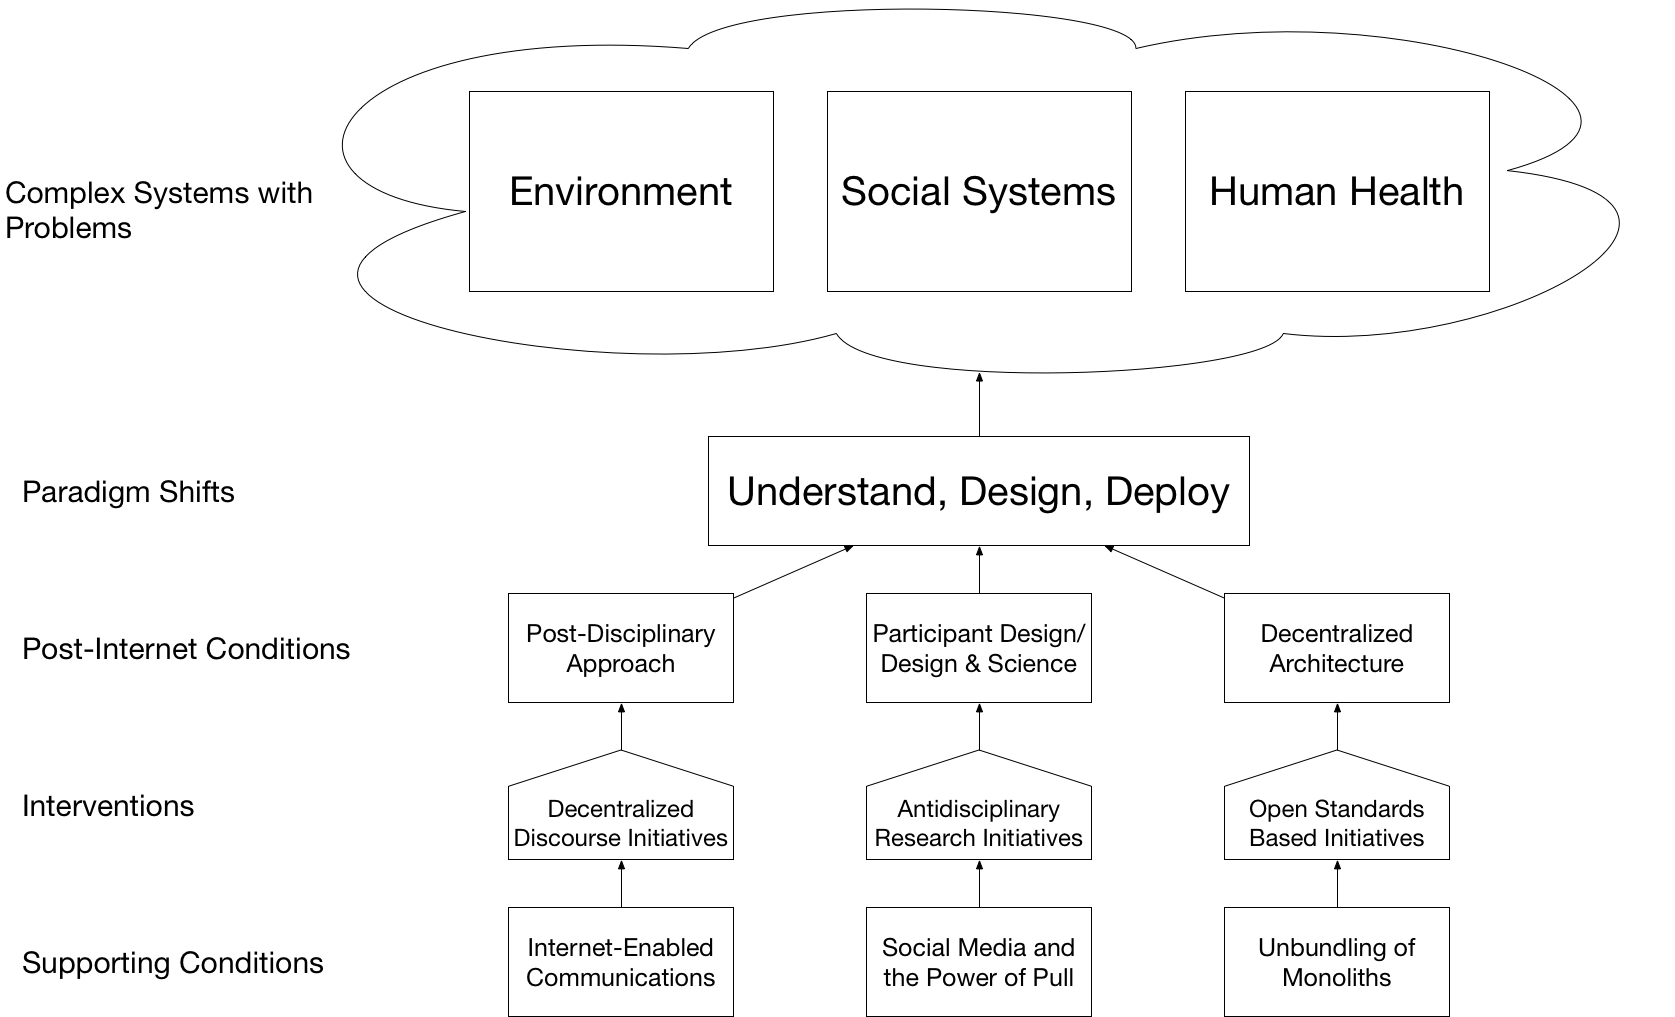
\includegraphics[width=1\textwidth]{pictures/TheoryOfChange}
 \caption[Diagram of my theory of change.]{My theory of change. In order to address the complex problems in the environment, social systems and human health, we must cause paradigm shifts to allow us to understand, design and deploy in complex systems. This paradigm shifts will require a post-disciplinary approach, a new participant design bringing together design and science and a decentralized approach with a decentralized architecture. These will require decentralized discourse initiatives, antidisciplinary research initiatives and open standards based initiatives. The Internet has caused new ways of communications, created social-media based organization models and provided a way for new open standards-based organization to break up traditional monolithic organizations.}
 \label{fig:theorychange}
\end{figure}

To address the problems in the environment, social systems and human health, we need a paradigm shift that allow us to understand, design and deploy interventions in complex systems. This paradigm shift will require a post-disciplinary approach; a new ``participant design'' process in which the participants in the system are the designers \cite{slavin_design_2016} (described more in \autoref{intro:design}); that brings together design and science; and a decentralized approach with a decentralized architecture. These in turn will require decentralized discourse initiatives, antidisciplinarity research initiatives, and open standards-based initiatives. We are ready for this paradigm shift because the Internet has created new forms of communications, social-media based organizational models, and the ability for new open standards-based organizations to break up traditional monolithic organizations.

I have long engaged in decentralized discourse initiatives --- that is, multi-way, open conversations that develop ideas and social relationships. As an early blogger (discussed in \autoref{sec:blogging}), I helped to bring blogs to Japan. Blogging inspired me to work on understanding emergent democracy (discussed in \autoref{sec:emergentdemo}). Some of my innovations in academic publishing include the \emph{Journal of Design and Science} and the MIT \ac{KFG} where we are experimenting with community and online-based publishing, challenging traditional academic publishing discussed in (\autoref{MITPress}). Also, the structure of the Media Lab that I am privileged to lead provides a decentralized, permission-free way to develop research and to carry on extended conversations about it (discussed in \autoref{antidisciplinaryapproach}).

Antidisciplinary research not only crosses disciplinary boundaries, but explores areas of research between and beyond disciplines that cannot be address by simple disciplinary intersectionality. For example, Health 0.0 reimagines diagnostics and therapeutics by fundamentally rethinking how we understand our biological systems, and by then developing and deploying technologies for treatment. This mirrors the way the Internet was developed by academics and grassroots communities outside of the incumbent industrial players (described in \autoref{sec:health00}). The Space Initiative is another example (described in \autoref{sec:spaceinitiative}). It takes advantage of the diminishing cost of space exploration and research to democratize participation in space exploration and research is. A third example is the Digital Currency Initiative at the Media Lab (described in \autoref{sec:DCI}). It aims at creating a core non-commercial, interdisciplinary, and antidisciplinary group to bring together and coordinate the development of standards and and technologies for digital currencies and the blockchain. It is situated in an academic environment, much like the early Internet was. Finally, the Ethics and Governance in Artificial Intelligence program --- the fund, course and research --- brings together all of the disciplines to forge a new interdisciplinary approach to thinking about and deploying artificial intelligence (described in \autoref{sec:EGAI}).

Examples of open standards-based initiatives include being the CEO of Creative Commons (described in \autoref{sec:CC}); being on the board of the Internet Corporation for Assigned Names and Numbers (ICANN); and being a board member of the Open Source Initiative described in \autoref{sec:OSI}. My commitment to open standards-based initiatives goes far back in my path. I helped set up and then served as the CEO of the first Internet service provider in Japan, PSINet Japan (described in \autoref{sec:PSI}). I co-founded Digital Garage, one of Japan's first web companies, which localized Infoseek Japan, one of the first search engines in Japan as well as providing other important Internet services. I advised and invested in in Havenco, an attempt to create an Internet hosting service outside of any government jurisdiction (described in \autoref{sec:havenco}). I have participated in the venture ecosystem first as an entrepreneur and later as an investor, with a primary interest in companies such as Flickr, Twitter and Kickstarter that have contributed to the Internet's open ecosystem.

\section{Understanding Change}
\subsection{Paradigms}
\label{intro:paradigms}

\marginpar{System dynamics and evolutionary dynamics can help us understand the dynamics of systems, as well as suggesting ways to intervene through a new design framework. One of the key insights of Meadows's work in systems dynamics is that the overall paradigms in a system drive the goals that then determine how elements in the system optimize. This view is consistent with evolutionary dynamics.}In his 1962 book, \textit{The Structure of Scientific revolutions}, Thomas Kuhn explains his idea of a ``paradigm'' by saying it is ``the set of common beliefs and agreements shared between scientists about how problems should be understood and addressed'' \cite{kuhn_structure_1970}. In a community or a social setting, paradigms can be the worldviews and values that silently shape thinking and research. From the perspective of systems dynamics, Donella Meadows says that the paradigm is that ``out of which the system --- its goals, power structure, rules, its culture --- arises.'' \cite{meadows_leverage}. Martin Nowak, director of the Program for Evolutionary Dynamics at Harvard, explains that in evolutionary dynamics and game theory, the paradigm determines the unit of payout for the game \cite{nowak2006evolutionary}. In a financial market system, for example, the payout is economic or financial gain. In biology, it is reproduction. Paradigms influence the fitness of strategies in evolution; the dynamics of communities; the behavior of complex adaptive systems, and what we can imagine and think. Paradigms can be transcended and altered, but there is no thinking outside of a paradigm.

System dynamics and evolutionary dynamics can help us understand the dynamics of systems, as well as suggesting ways to intervene through a new design framework. One of the key insights of Meadows's work in systems dynamics is that the overall paradigms in a system drive the goals that then determine how elements in the system optimize. This view is consistent with evolutionary dynamics.

\subsection{Systems Dynamics}

Climate change and disparities in health and income are highly complicated problems. Each is, in fact, a complex adaptive system, which means that its vitality and flourishing are not improved by working harder, doing more, or scaling. In the field of systems dynamics, which explores managing complex systems, the positive feedback systems that create exponential growth and that have the highest business payouts are typically viewed with alarm rather than envy because they tend to lead to unsustainable growth and ecosystem collapse.

\marginpar{Climate, health and income disparity are highly complicated problems. Each is, in fact, a complex adaptive system, and their vitality and flourishing are not improved by working harder, doing more or scaling.}The field of system dynamics was developed in the 1950s by Professor Jay Forrester of MIT. In 1972, the Club of Rome commissioned systems dynamics researchers to create a computer simulation of exponential growth in an environment of limited resources. The model used five variables, each growing exponentially: ``population, food production, industrialization, pollution, and consumption of nonrenewable natural resources.'' The report was called ``The Limits to Growth.'' Two scenarios showed ``overshoot and collapse'' in the 21st century, and one showed stabilization \cite{meadows_limits_2004}. Research continues in understanding resilience and the similarities between social systems and ecosystems \cite{folke2006resilience}. 

A simple system looks something like this (see \autoref{fig:meadows}).

\begin{figure}[h]
 \centering
 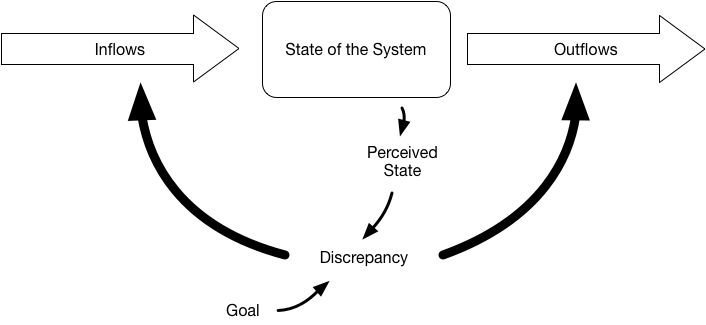
\includegraphics[width=1\textwidth]{pictures/System.png}
 \caption{Image of a simple system inspired by figure from Donella Meadows's essay \cite{meadows_leverage}}
 \label{fig:meadows}
\end{figure}

The state of the system, or the ``stock,'' is like the amount of money in an account, the amount of water in a lake, the amount of CO$_2$ in the atmosphere, or even the amount of trust in a government. Let's take the water in a bathtub as our example of stock. The inflows are the water flowing from the faucet. The outflows are water flowing out of the drain. By closing the drain and turning on the faucet, you can get the water, or stock, to increase in the tub. The ``goal'' is to get the right amount of water into the tub. You can watch the water level and control the inflow by turning on the water, or, if you end up with too much water after you sink into the tub, you could open the drain and lower the water level. It's apparent that it will be hard to control the water level of a tiny tub with a faucet connected to a fire hose, and that a large, overflowing tub of scalding water with a tiny drain will take a long time to cool.

Now imagine that you want to control the temperature. You might add hot water. But the boiler is far away in the basement,  so there is a delay after you turn the hot water knob. Then imagine the system that gets the water to your apartment and the system of energy behind the boiler. The energy might  come from a utility that provides you energy, but depletes your bank account. The goal of the utility is likely different than your goal when you are filling the tub for a nice warm bath: their goal may be to maximize their profits and take as much money from you as possible without depleting your bank account completely. The system gets complex quickly, especially since everything is interconnected...and the different systems may well have different goals.

See figure \autoref{fig:3sys} for an example of three systems connected together and \autoref{fig:9sys} for an example of nine systems connected together. Figure \autoref{fig:metasys} shows systems of systems connected together.


\begin{figure}[h]
 \centering
 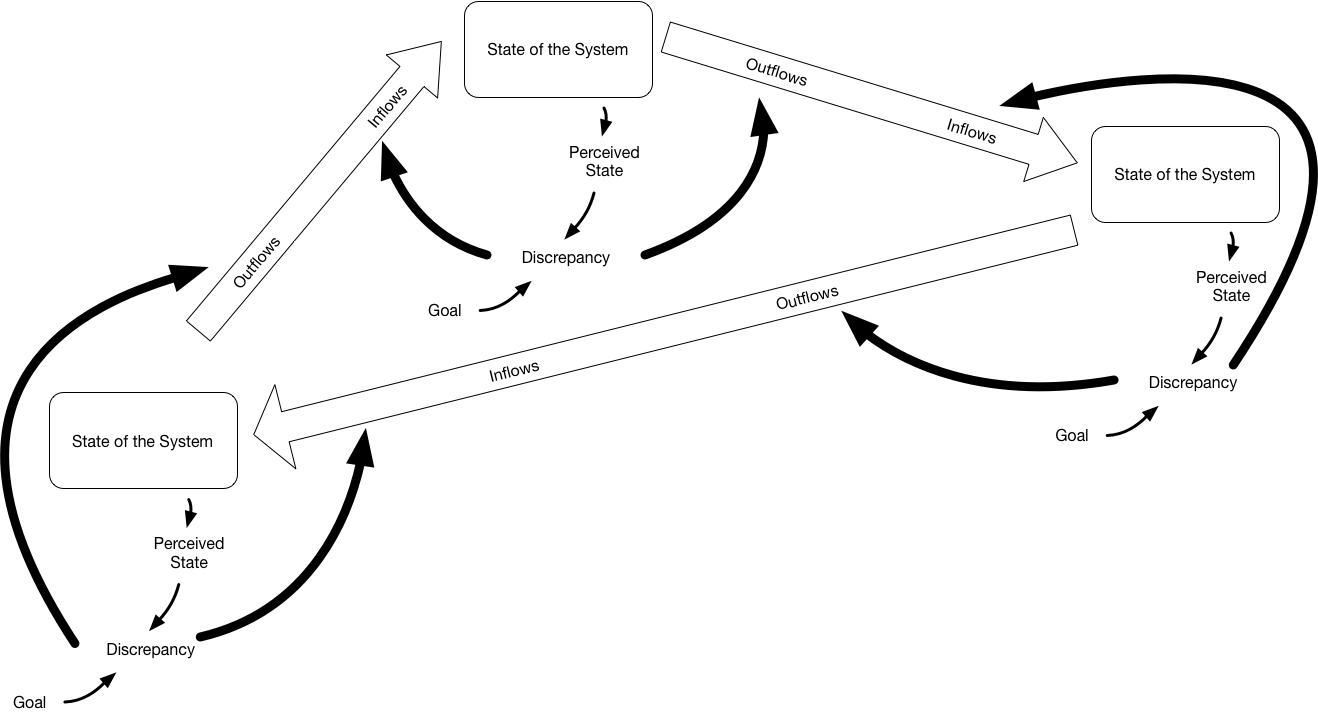
\includegraphics[width=1\textwidth]{pictures/3sys}
 \caption{Three systems connected together.}
 \label{fig:3sys}
\end{figure}

\begin{figure}[h]
 \centering
 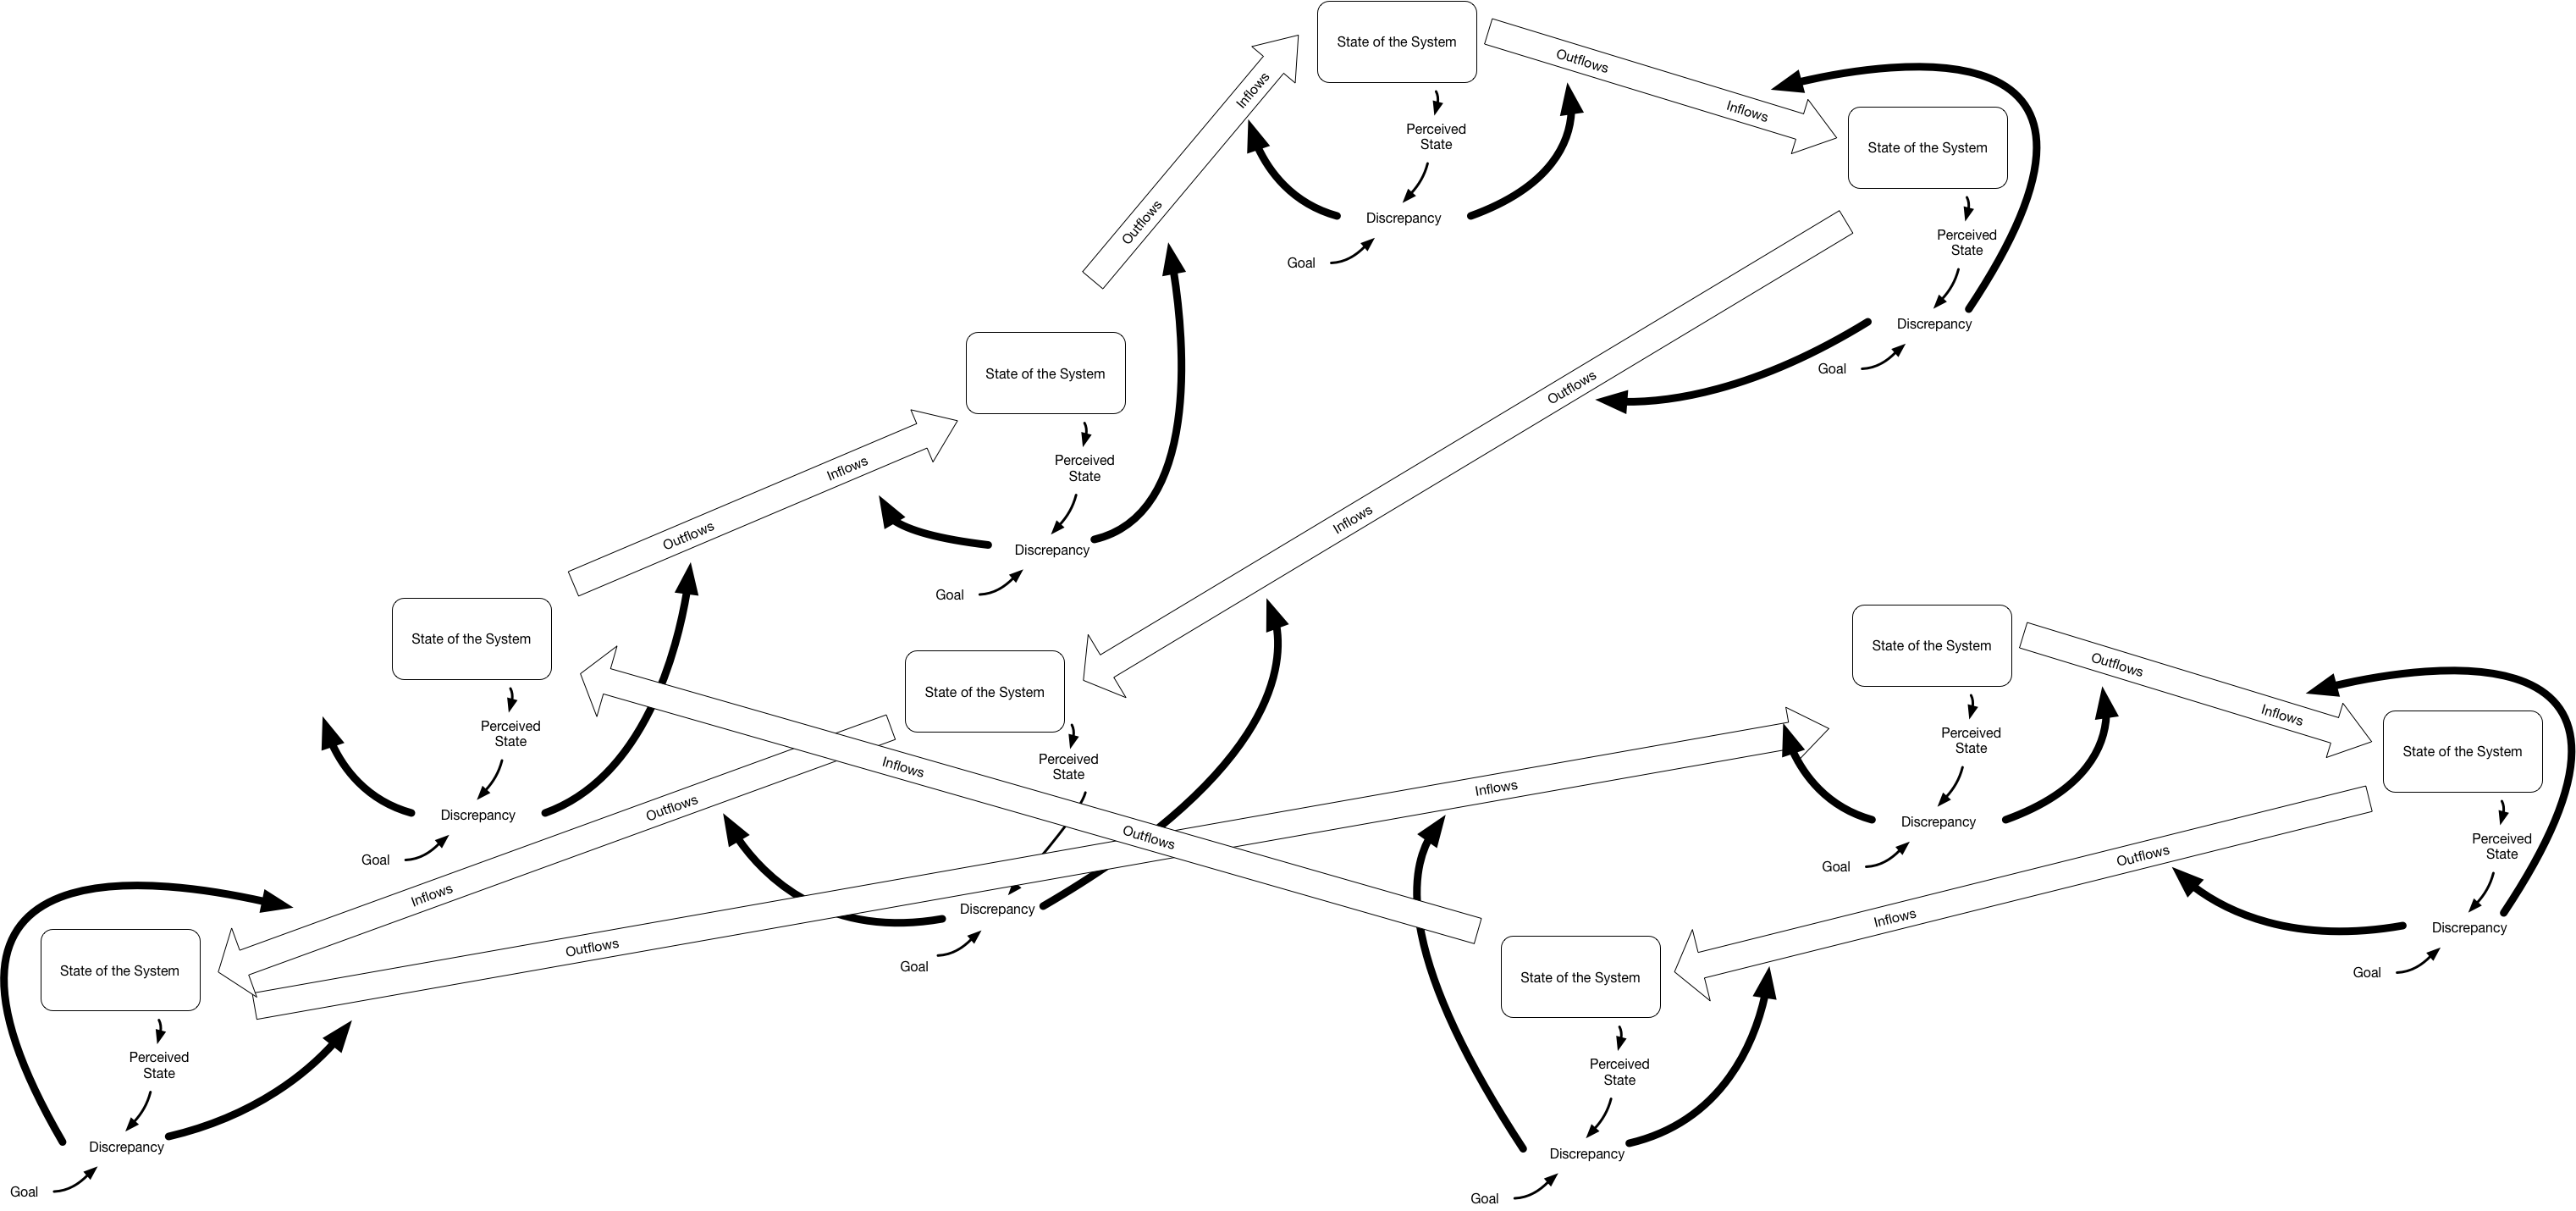
\includegraphics[width=1\textwidth]{pictures/9sys}
 \caption{Nine systems connected together.}
 \label{fig:9sys}
\end{figure}

A cell is a system with goals, and the human body is a system of cells with our own goals. Society is a system of individuals, communities, cultures, corporations etc. The planet is a system of societies, geological systems, other organisms, etc. Everything is a system of interconnected systems across scales.

\begin{figure}[h]
 \centering
 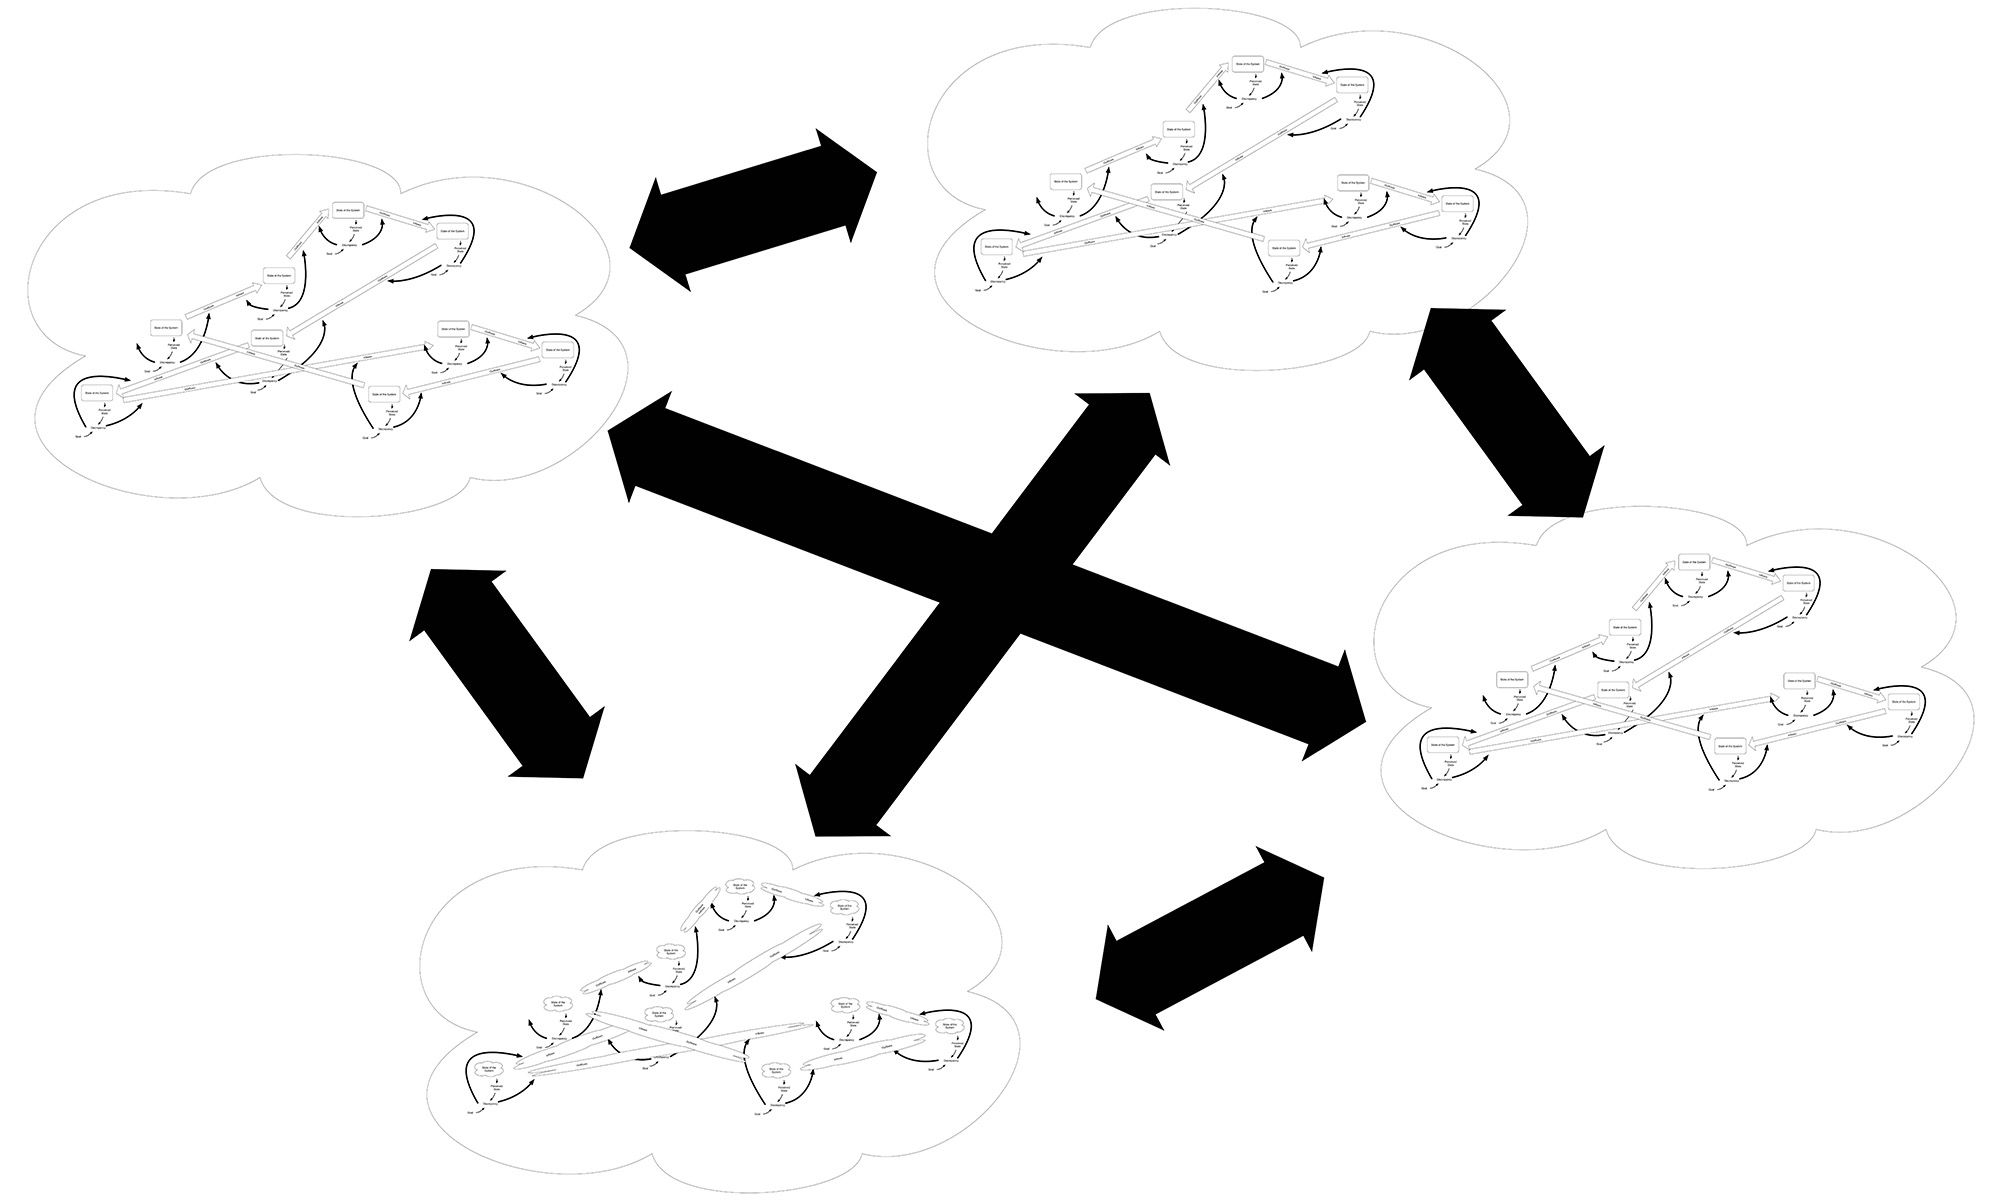
\includegraphics[width=1\textwidth]{pictures/metasys}
 \caption{A system of systems.}
 \label{fig:metasys}
\end{figure}

\subsection{Evolutionary Dynamics}
\label{intro:evolution}

\begin{figure}[h]
 \centering
 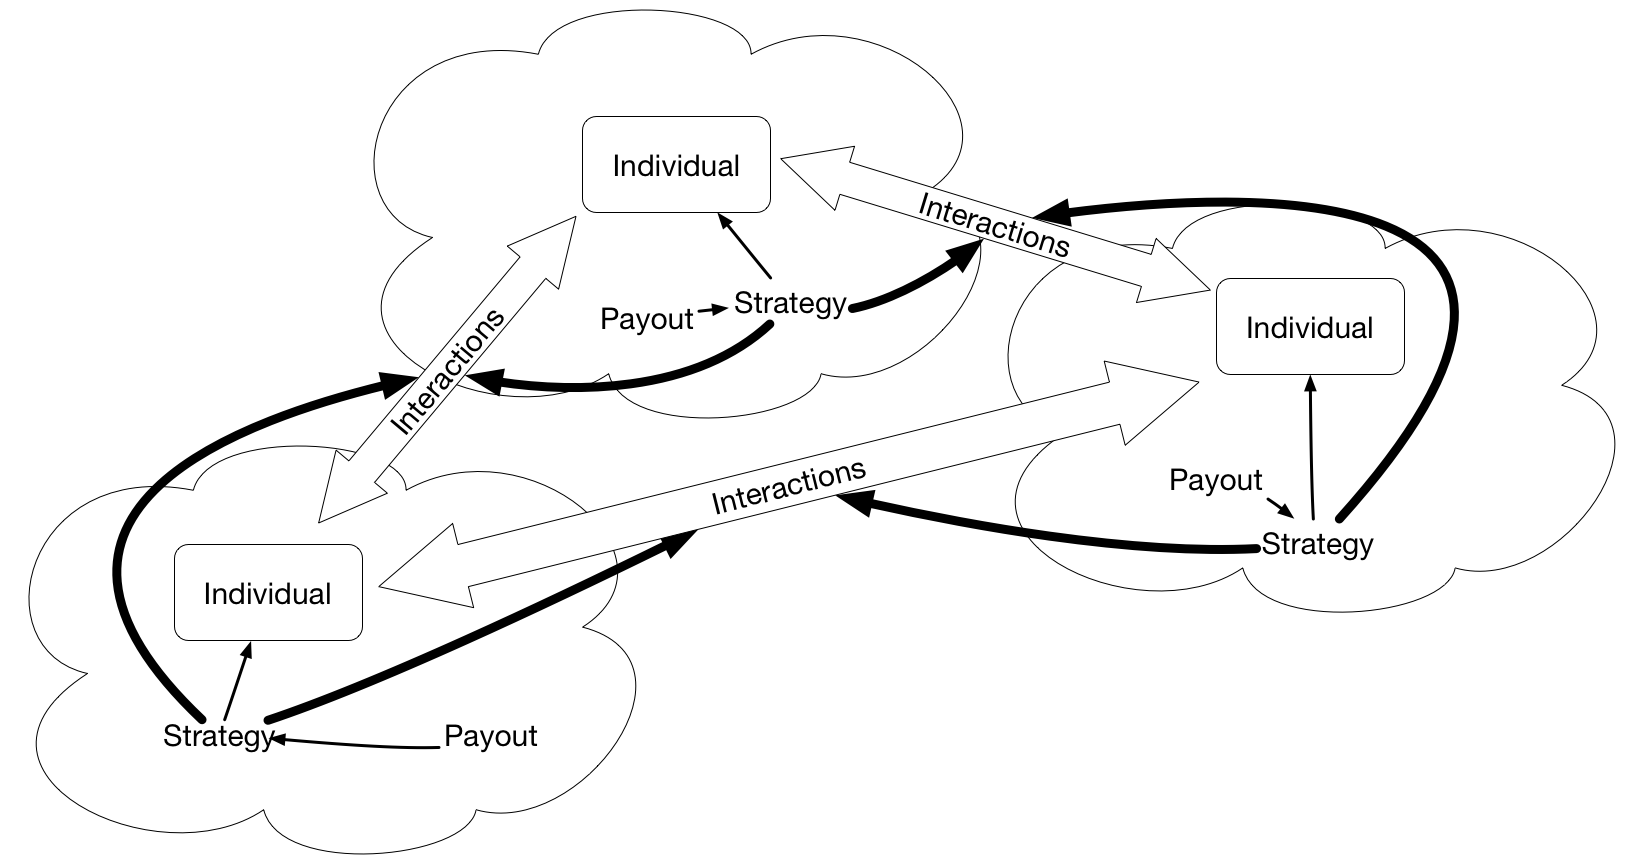
\includegraphics[width=1\textwidth]{pictures/EvolutionarySystem}
 \caption[Evolutionary dynamics version of interacting systems.]{Evolutionary systems look a lot like systems as described in systems dynamics, except that evolutionary dynamics does not use the term ``goals''. Instead individuals in a population interact with each other based on a strategy. This strategy optimizes for a payout from a ``game'' and the strategy evolves over time as the strategy of the other individuals change. \cite{nowak2006evolutionary}}
 \label{fig:evolution}
\end{figure}

While systems dynamics is useful in understanding the relationships between systems and how they behave, evolutionary dynamics is useful in understanding how systems evolve over time. (See figure \autoref{fig:evolution}.) Evolutionary dynamics is the evolutionary outcome of increasingly effective strategies individuals use to optimize for maximum payout \cite{nowak2006five, nowak2006evolutionary}. The payout is the measurement of the success and the fitness of a strategy; it is defined by the paradigm. Material value has been quantified by the emergence of money and the economy. The field of economics is able, through the utility function, to quantify in economic terms even immaterial payouts. While this is rational, humans have bounded rationality, and in practice, that has required traditional economic models to be reductionist.

The reducibility of norms into a utility function and economic motivation has been questioned by economists \cite{kreps1997intrinsic}. Workers who have internalized a company's welfare may get confused when extrinsic motivators in the form of economic incentives are implemented \cite{ichniowski1995effects}. Another experiment showed that people being paid to assemble Lego blocks would assemble more if the completed models were preserved rather than disassembled each time \cite{ariely2008man}. Individuals try to find meaning in even seemingly meaningless tasks, and are motivated in non-financial ways.

This evidence not withstanding, economists and business leaders continue to focus on financial extrinsic motivation as the key method for managing behavior. This necessarily reduces the diversity of strategies and decreases the robustness of our ecosystem. My argument is that the most difficult problems we face today --- climate change, global income disparity, and public health --- are a result of the effectiveness of solutions that maximized short-term payouts that we can measure and enjoy within our bounded rationality and perspective. Climate change can be directly linked to the success of industry in creating abundance at the expense of nature by exploiting and extracting resources. Much of modern chronic disease comes from agricultural gains that have made food abundant and cheap, and all manner of conveyance ensures we no longer need to walk and forage. The capital markets have become so efficient that passive capital continues to yield more and more returns, extracted from workers and society that are exceedingly underrepresented in setting strategy and participating in the payouts. There are, of course, ideas like the triple bottom line \cite{hall2011triple} and other attempts to nudge actors in markets to think longer term and behave more socially responsibly. While these attempts are an important move in the right direction, markets overall continue to optimize on shorter and shorter time scales, extracting more and more value from the future --- metaphorically very similar to the climate issue.


\subsection{Cybernetics}
\label{intro:cybernetics}

The Cold War era was defined by the rapid expansion of capitalism and consumerism, the beginning of the space race, and the dawning of the age of computation. It was a time when it was easier to believe that systems could be controlled from the outside and that many of the world's problems would be solved through science and engineering.

The cybernetics that Norbert Wiener and others described \cite{wiener1961cybernetics} during that period was concerned with feedback systems that can be controlled or regulated from an objective perspective. This so-called first-order cybernetics assumed that a scientist as an observer can understand what is going on, and therefore an engineer can design systems based on observations and insights from the scientist.

In the late 60s and early 70s, Margaret Mead, Heinz von Foerster, and others developed the notion of second-order cybernetics \cite{glanville2002second}: the cybernetics of cybernetics. Second-order cybernetics described adaptive complex systems, where the scientist-observer is part of the system itself.

While the study of systems dynamics and cybernetics continues, cybernetics reached an apex during a famous series of interdisciplinary meetings held between 1946 and 1953 as part of the Macy Conferences. The use of the word ``cybernetics'' in books peaked around 1969 (\autoref{fig:cybernetics}). Both cybernetics and systems dynamics flourished when they had heavy interdisciplinary participation and real impact. How disciplines and the communities that support them emerge and wither is a key topic of this dissertation, and the study of systems is a great example of numerous communities and approaches.

\begin{figure}[h]
 \centering
 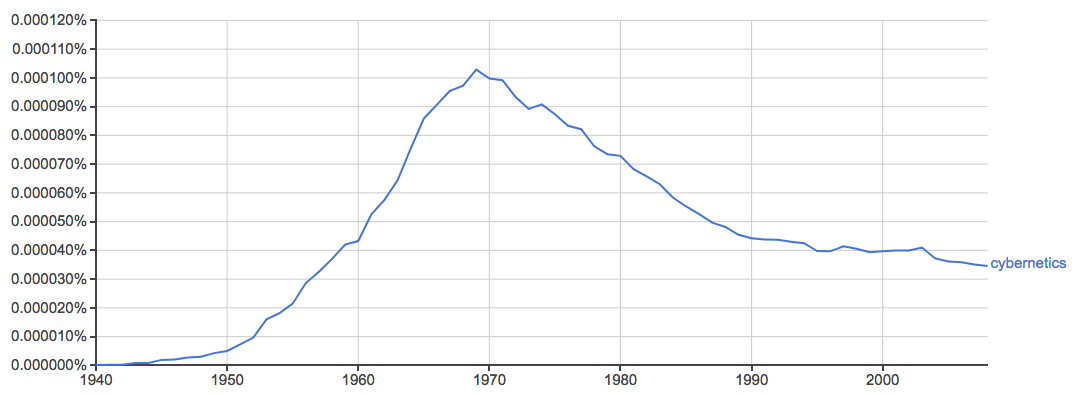
\includegraphics[width=1\textwidth]{pictures/cyberneticsuse}
 \caption[Graph of the use of the word ``cybernetics'' in books from 1940-2018 according to Google Books.]{Graph of the use of the word ``cybernetics'' in books from 1940-2018 according to Google Books. The word ``cybernetics'' increases in use rapidly after World War II peaking in 1969 with a steady decline for a few decades and leveling off.}
 \label{fig:cybernetics}
\end{figure}

We now have an opportunity and an imperative to pull the disciplines together again in the context of our new tools and our new challenges, and to tackle the wicked problems.

\subsection{Solving Complex Problems}

While systems dynamics and cybernetics have helped us model and understand complex problems, the really big and complex problems were described as ``wicked problems'' by Horst Rittel and Melvin M. Webber in ``Dilemmas in a General Theory of Planning.'' \cite{rittel_dilemmas_1973} They explain that these problems are beyond our ability to ``solve.'' ``Moreover, because of complex interdependencies, the effort to solve one aspect of a wicked problem may reveal or create other problems'' \cite{rittel_dilemmas_1973}.

Donella Meadows, a colleague of Jay Forrester at MIT who worked on the model for the Club of Rome previously described, proposed a way forward in her essay, ``Leverage Points'' \cite{meadows_leverage}. She suggests that since the goals of a system are generated by its paradigm, the ability to transcend the paradigm provided the most leverage for intervening in complex systems.

\section{Designing Change}
\subsection{Design}
\label{intro:design}

Most of what we design involves some part of a complex system such as the system that gets water into and out of a bathtub, but we usually just assume those support systems rather than focusing on them. For example, modern design is usually focused on the customer and the customer experience. For example, many ``Uber for food'' services like Doordash are a great experience for the customer. You have an app, you click it a few times to order food and before you know it, it's at your door. But what about the driver, the cook in the restaurant... what's the experience like for them? How much attention did the app developers give to their experience?

In the article ``Why I Quit Ordering From Uber-for-Food Start-Ups'' \cite{sloan2015quit} in \textit{The Atlantic Magazine}, Robin Sloan argued that the cooking/food service startup Josephine was better than food delivery services because it was designed for chefs as well as for customers. Josephine matched people who like to cook food in their homes with people in the neighborhood willing to pay to eat the food the home cooks made. This service was designed for the consumer \textit{and} the producer, and it also worked to promote a healthier neighborhood. The entrepreneurs behind Josephine looked at more of the system, not only the subject of the consumption. And that system is even more complex than Josephine recognized. It includes not only all humans in the neighborhood, but also the food supply chain, the food waste chain, and many other things that could be designed for as well.

\marginpar{In the \textit{Journal of Design and Science}'s first article, ``Design as Participation,'' \cite{slavin_design_2016} Kevin Slavin uses the quote ``you're not stuck in traffic, you are traffic.''}In the \textit{Journal of Design and Science}'s first article, ``Design as Participation,'' \cite{slavin_design_2016} Kevin Slavin uses the quote ``you're not stuck in traffic, you are traffic.'' Josephine was designed by people who understood home cooking aficionados and were closer to the system. But ultimately, if you really want to understand the system, you have to be part of the system. The design of a healthy complex system requires designers to be both observers of a system and humble participants in it.

At MIT, professors Neri Oxman and Meejin Kim teach a class called Design Across Scales. In this class, they describe systems at every scale, from the microbial and human to the architectural and urban to global and astronomical systems, and they demonstrate how all of these system are connected. Most scientists and designers are focused on a single scale and a single system, when instead they can and must understand how their work connects to and affects all systems at all scales and take responsibility for their interventions into these systems.

In ``Age of Entanglement,'' Oxman presents the Krebs Cycle of Creativity \cite{oxman_entanglement_2016}. This illustrates science adopting the perception of nature and converting it into knowledge. Engineering takes this knowledge and converts it into utility. Design takes this knowledge and converts it into meaning, behavior, and societal value. Art takes it and converts it into social perception. And although it's too rare, this should be in the input into science as well. My view is that science, engineering, design, and art need to work seamlessly together in order for creativity to be well expressed.

\begin{figure}[h]
\centering
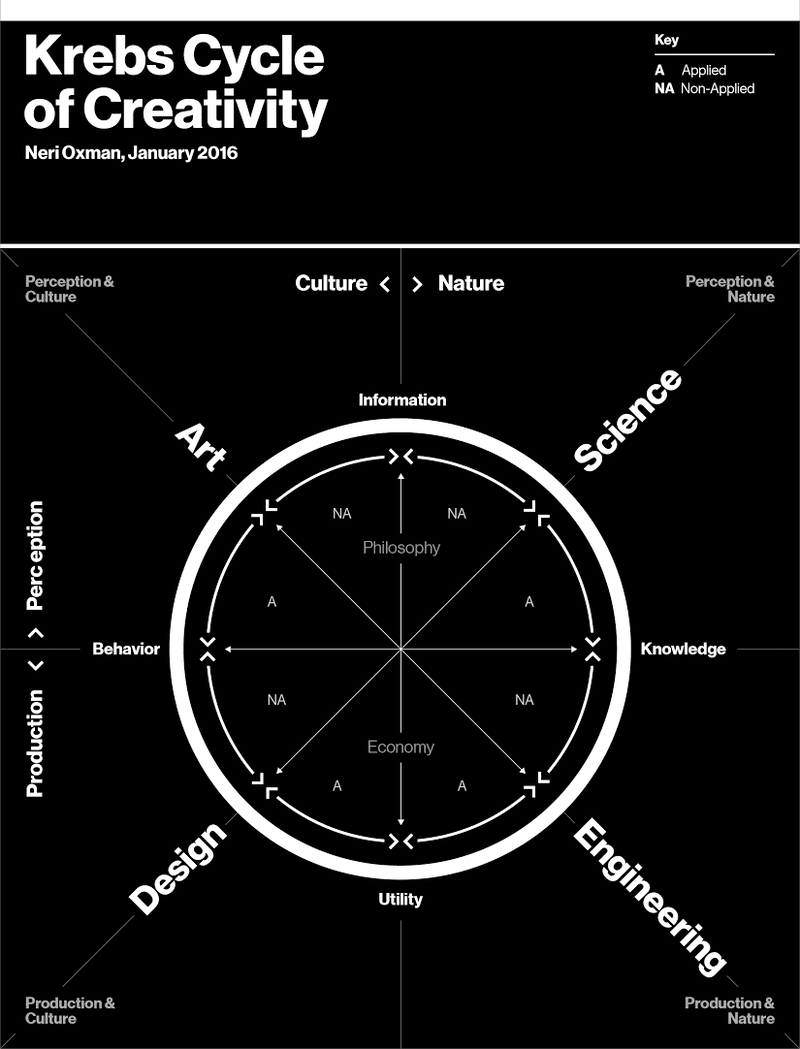
\includegraphics[width=.5\textwidth]{pictures/krebs.eps}
\caption{Krebs Cycle of Creativity \cite{oxman_entanglement_2016}}
\label{fig:krebs}
\end{figure}

In Oxman's Krebs Cycle of Creativity (\autoref{fig:krebs}), the relationship between the disciplines, design and science are opposite one another on the circle, and the output of one is not the input of the other as is often the case with engineering and design, or science and engineering. I believe that through the fusion of design and science, we can fundamentally advance both and provide ourselves with a new ``lens'' to view systems. This connection includes both the science of design and the design of science, as well as a dynamic relationship between these two activities.

I am using the term ``science'' to mean the study of biological and other hard sciences, whereas I mean ``design'' as a way to develop interventions in the environment and complex systems, in contrast to more tradition definitions of ``design science,'' which focuses on the methodological understanding of design as a process \cite{cross2001designerly}.

Much of design in the past was about the  visual and aesthetic. Modern design brought together form and function. In the 1896 paper ``The tall office building artistically considered,'' Chicago architect Louis Sullivan first proposed the notion of form following function \cite{sullivan1896tall}. Design and engineering came together to bring a social sensibility to the design of technologies from the mouse to user interfaces, from the physical to the immaterial. 

Today, many designers work for companies and governments, developing products and systems focused primarily on ensuring that society works efficiently. However, the scope of these efforts is not designed to include --- or care about --- needs beyond those of corporations or governments. We're moving into an era where the boundaries of various systems are not so defined. Systems such as the microbial system and the environment have suffered and now present significant challenges for designers. With such adaptive and complex systems, our unintended effects on them often produce unintended negative consequences for us.

\marginpar{Designers are not just planners wielding deterministic tools and control, but rather are participants in vast systems in which they exist and participate. This requires designers to employ a much more humble, non-deterministic approach and requires scientists and engineers to think across multiple scales and systems with greater intent and sensibility.}Designers are not just planners wielding deterministic tools and control, but rather are participants in vast systems in which they exist and participate. This requires designers to employ a much more humble, non-deterministic approach and requires scientists and engineers to think across multiple scales and systems with greater intent and sensibility. In ``Inviting Feedback'' in the \textit{Journal of Design and Science}, Pip Mothersill points out that, ``We don’t just design forms, we now design platforms'' \cite{mothersill_inviting_2018} and that those designing such platforms are designing ecologies.

Traditionally the domain of designers alone, this sensibility is a kind of aesthetic, though not merely a visual one. Rather, the field of design is trying to evolve beyond its traditional concern with visual aesthetics, and begin adopting a more philosophical aesthetic or sensibility, one more like that of indigenous peoples. The solution to the climate problem isn't more productivity, it is instilling a sensibility that ``more than enough is too much.'' Many of our contemporary health problems emerge from convenience, which is a modern commercial value that had no value at all in the rituals of the past. Income disparity is in many ways a function of a highly efficient capitalist system that rewards owners of resources, putting growth and progress above all else, and that exploits nature --- all concepts foreign, and even abhorrent, to many indigenous cultures, such as Polynesians and Native Americans, for example.

As we try to address problems like climate change or redesign systems like the criminal justice system, in the age of \ac{AI} such sensibilities and aesthetics are more important than compositional and structured tools like A/B testing or the economic models we currently rely on to shape our world. The linear and logical decision-making design that Herbert Simon describes in ``The Sciences of the Artificial'' \cite{herbert1978science} seems too reductionist for our complex problems. However, we must also be careful that our haste to resist reduction and structure does not lead to the ``structurelessness'' that resulted when the feminist movement rejected the idea of leaders, and thereby ended up with an informal and less accountable form of leadership, as described by Jo Freeman in ``The Tyranny of Structurelessness'' \cite{freeman1972tyranny}.

\marginpar{We must accept that the outcome of more and more scientific and technological design will not be fully in our control. It will instead be more like giving birth to a child and influencing its development. My work as director of the MIT Media Lab is to foster and nurture the use of respectful design in science and technology so that we enhance and advance the complex, adaptive systems we live within.}We must accept that the outcome of more and more scientific and technological design will not be fully in our control. It will instead be more like giving birth to a child and influencing its development. My work as director of the MIT Media Lab is to foster and nurture the use of respectful design in science and technology so that we enhance and advance the complex, adaptive systems we live within. 

\subsection{The End of the Artificial}

Unlike the past when distinct boundaries separated the artificial and the organic, the cultural and the natural --- science explored the natural and engineering built the artificial --- now it appears that nature and the artificial are merging.

Science and engineering today are delving into synthetic biology and artificial intelligence, which are both massively complex. These new areas of study and exploration necessarily take engineers out of the domain of the artificial and scientists into the domain of the natural. We are increasingly able to design and deploy directly into the domain of ``nature'' and in many ways ``design'' and ``edit'' nature. We have machine learning models that are exhibiting unpredictable and unexplainable behavior on the one hand. On the other hand, we are starting to see order in biology where we expect randomness. For example, while scientists argue that biology is inherently stochastic at the molecular level, research led by Deblina Sarkar has revealed nanoscale alignment of biomolecules in synapses between different neurons in brain that can not be explained without some coordinating and “ordering” mechanism, details of which are still unknown \cite{Sarkar2018}. We are therefore finding unexplainable order at the bio-nano-scale and unexplainable complexity at the digital-scale.

\subsection{Disciplines and Scholarship}
\label{intro:disciplines}

\marginpar{As we bring the artificial and the natural together and integrate the work of designers, artists, engineers, and scientists, the inability of academic disciplines to communicate with each other and our own difficulties conceiving ideas across disciplinary boundaries become significant impediments.}As we bring the artificial and the natural together and integrate the work of designers, artists, engineers, and scientists, the inability of academic disciplines to communicate with each other and our own difficulties conceiving ideas across disciplinary boundaries become significant impediments.

Linguistic relativists argues that language determines what one can think. This theory is controversial, but studies have shown that language does affect how we perceive color \cite{kay_paul_what_2009} or how we understand math \cite{everett_linguistic_2011, holden_life_2004}. If mathematics and mathematical symbols are a language, it is one that clearly limits or augments what we can imagine and discuss \cite{saxe_cultural_2012}. Michel Foucault, the French philosopher who pioneered modern thinking about the relationship between knowledge and institutional power, used the term ``épistémè'' to describe the space of possible, knowable things due to the rules and constraints of the language \cite{foucault_order_2002}. Foucault argued in \emph{Archeology of Knowledge} \cite{foucault_archaeology_2002} that knowledge is generated through discourse governed by the rules of institutions and the relationship between individuals. This is aligned with Kuhn's idea of paradigms as explained in\emph{The Structure of Scientific Revolutions} \cite{kuhn_structure_1970}: paradigms as linguistic formulations as well as codes of practice direct what and how knowledge is created and understood. \emph{Science in Action}. Before both Foucault and Kuhn, Ludwig Fleck, a Polish microbiologist and philosopher, had in the 1930s and 1940s described ``thought collectives'' as groups of people whose knowledge exists only because they are within the context and epistemology of that group \cite{fleck_entstehung_1979}.

Martin Nowak shows mathematically how learning from examples, or inductive inference, requires constraints \cite{nowak_computational_2002}. These constraints include the language constraints acquired by cultural evolution and the biological evolution of universal grammar \cite{chomsky_minimalist_1995}. In other words, you cannot learn anything through inference without constraints such as language. Indeed, Yuval Noah Harari, the Israeli historian argues in \textit{Sapiens} that ``the truly unique feature of our language is not its ability to transmit information about men and lions. Rather, it's the ability to transmit information about things that do not exist at all'' \cite{harari_sapiens:_2015}. So, we may need language even to conceive of that which is not there.

 \cite{latour_science_1987}, Bruno Latour, a French philosopher, argued that facts became facts through citation. Citations help form boundaries around disciplines, and simultaneously favors points of view that fit within the existing corpus, not ideas that question established theories and opens black boxes. Citations, according to Latour, serve a political purpose within disciplines. In ``Situated Knowledges: The Science Question in Feminism and the Privilege of Partial Perspective'' \cite{haraway_situated_1988}, Donna Haraway goes a step further, arguing that all knowledge is the result of ``power moves'', not moves towards truth. Disciplines under this analysis look like they are about power, not just knowledge.

So: academic disciplines are thought collectives with their own paradigms and specialized languages. Peer review reinforces adherence to those rules, paradigms, and patterns of language. The social dynamics that arise from the relationships among individuals in a discipline and the way funding and acknowledgement flow further reinforce the episteme, isolating disciplines from interaction with other disciplines. Disciplines package knowledge into bricks and black boxes \cite{latour_pandoras_1999} that may be used by other disciplines or subdisciplines without understanding the inside of the bricks themselves. Opening such black boxes and understanding what's inside is required for paradigm shifts and ``epistemological rupture'' \cite{bachelard_formation_2002} --- but that requires significant social and financial resources \cite{latour_science_1987}. Thus, the old adage, ``we are getting to know more and more about less and less'' \cite{fowler1911religious} is increasingly true. 

Approximately 2.5 million scientific papers are published each year \cite{jinha_article_2010}. In 2009, we passed the fifty million mark for the total number of science papers published since 1965. Fewer than one percent of scientists, however, publish a paper each year \cite{stokstad20141}. Just reading all the papers in a single discipline has become humanly impossible --- and publications represent only a small amount of the work in a field.

We clearly need to reconsider the way we develop knowledge and communicate within a discipline as well as between disciplines.

Interdisciplinary work has produced impactful results. Robert Langer, one of the most cited engineers in history \cite{noauthor_2610_2018}, helped bring engineering and biology together, creating the interdisciplinary field of bioengineering \cite{noauthor_struggles_2012, pearson_profile:_2009}. Multidisciplinary work has become much more common as computer science, engineering and other fields have converged to produce valuable results. However, these efforts suffer from lengthy and complicated beginnings; have difficulty finding funding; and require quite a bit of risk on the part of researchers who venture into research areas with no peers, no journals and often no obvious academic home.

\subsection{Rethinking the Disciplines}
\label{chap3:antidisciplinary}

\begin{figure}[h]
 \centering
 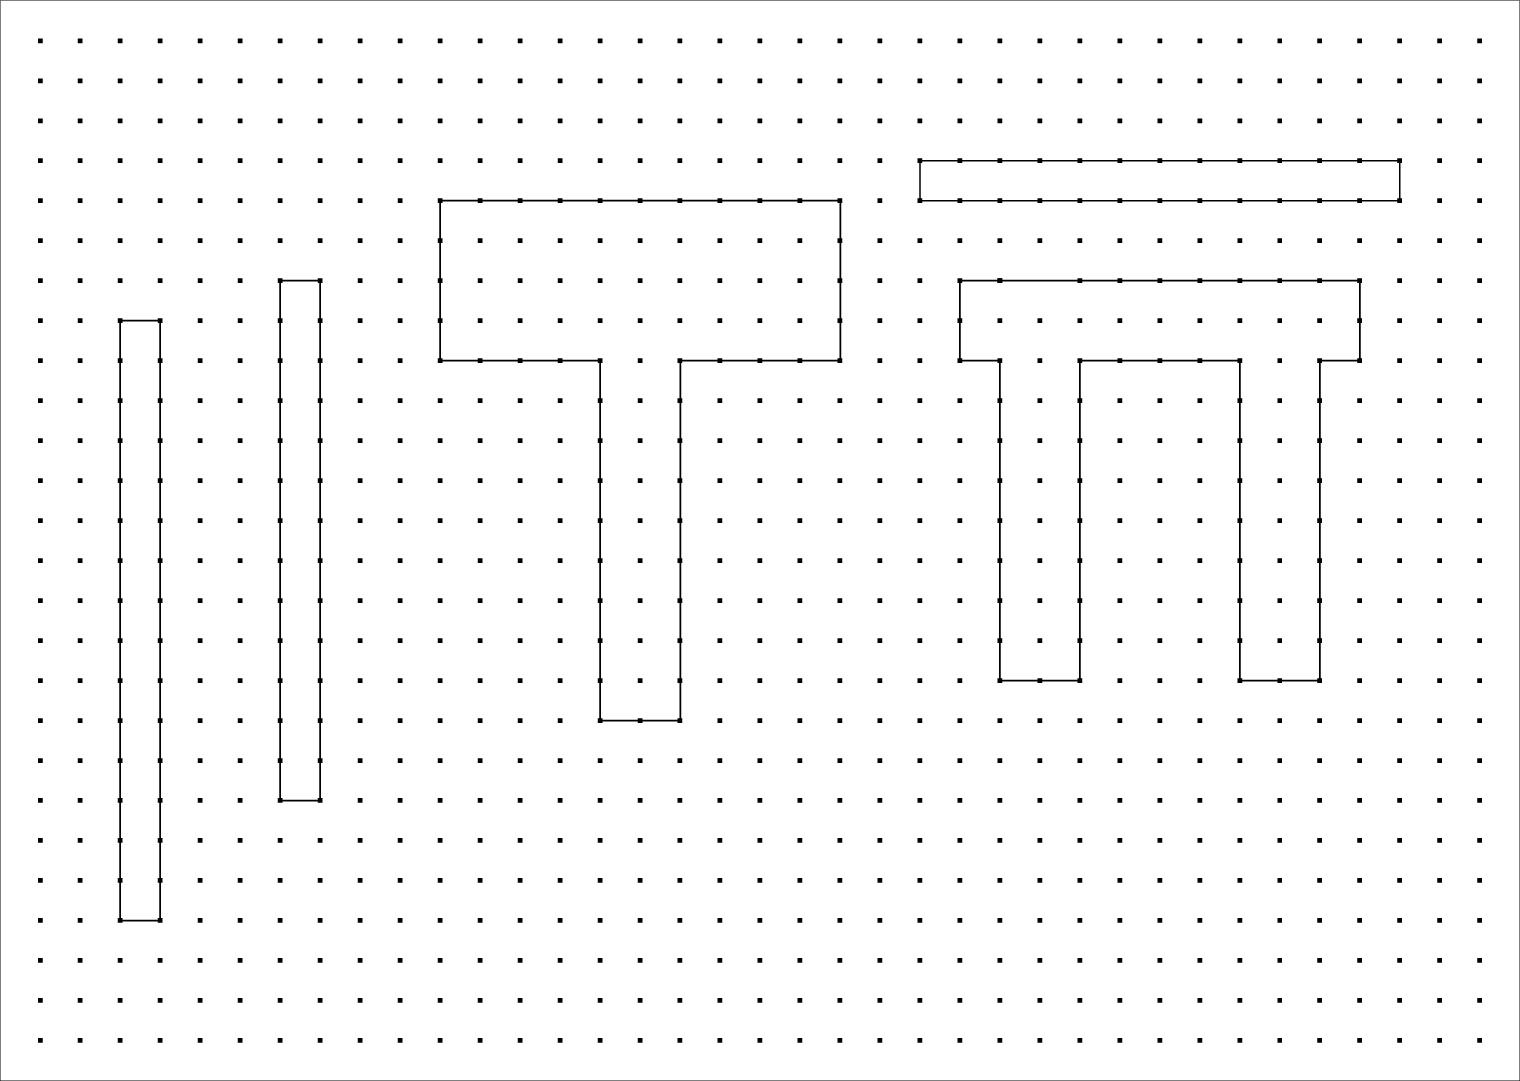
\includegraphics[width=1\textwidth]{pictures/JoiIllustr_V3-01.jpg}
 \caption[Image of shapes of disciplinary specialization.]{The vertical axis is depth. The horizontal axis is breadth. The horizontal line is normal non-academic people who follow the news. ``I'' people and specialists who go deep but can't explain what they do the the public. Some are specialists who can talk to the public but are sometimes less deep. ``T People'' are relatively deep but can talk broadly. Some people are ``$\pi$ People'' who are interdisciplinary.}
\label{fig:discipline001}
\end{figure}

\begin{figure}[h]
 \centering
 
\includegraphics[width=1\textwidth]{pictures/JoiIllustr_V3-02.jpg}
 \caption{``Multi-disciplinary people'' or ``M'' people are deep in more than two disciplines.}
 \label{fig:discipline002}
\end{figure}

\begin{figure}[h]
 \centering
 
\includegraphics[width=1\textwidth]{pictures/JoiIllustr_V3-03.jpg}
 \caption{``M'' people can bridge people who are specialists in other disciplines.}
 \label{fig:discipline003}
\end{figure}

\begin{figure}[h]
 \centering
 
\includegraphics[width=1\textwidth]{pictures/JoiIllustr_V3-04.jpg}
 \caption{``Antidisciplinary people'' are also looking for opportunities between the disciplines.}
 \label{fig:discipline004}
\end{figure}

\begin{figure}[h]
 \centering
 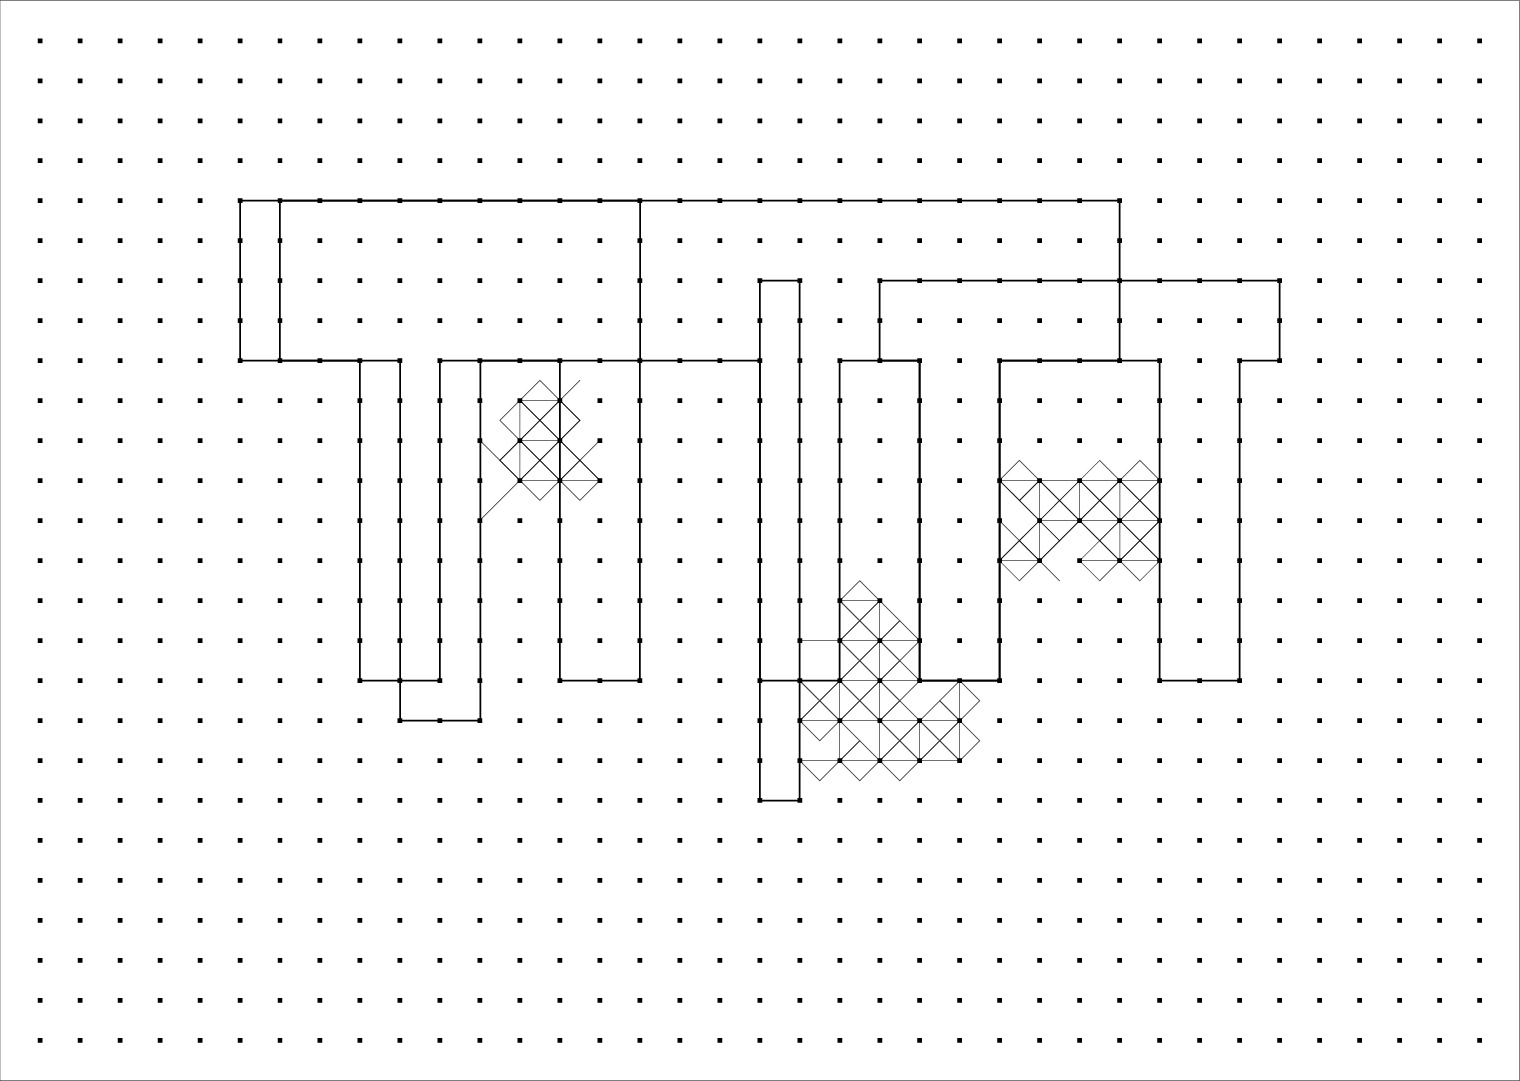
\includegraphics[width=1\textwidth]{pictures/JoiIllustr_V3-05.jpg}
 \caption{A diverse combination of I, T, $\pi$, multi-disciplinary and antidisciplinary people create a vibrant ecosystem of depth,breadth, and emergent disciplinary interactions.}
 \label{fig:discipline005}
\end{figure}

People who conduct research can be modeled as individuals in a population in an evolutionary dynamics game. While academics do care about money, their payout is often success in some combination of impact, peer validation, and the joy of discovery. While economists can model all of these payouts as a form of utility function that can ultimately be converted to monetary value, few academics calculate the dollar value of each citation when they write a paper. They are more likely thinking about their progression through the academic system, heading toward a degree or tenure. They are also likely to be thinking about power and funding (getting closer to a utility function calculus), which will allow them to hire researchers and buy equipment and materials to conduct experiments that incrementally augment or perhaps overturn existing theories.

In this way, the structure of academic institutions, with their schools and departments providing degrees and tenure through a process of peer review, reinforces the focus on going deeper rather than wider --- the target of the work of most academics focusing on a very small number of people who are sufficiently advanced in a field to understand whether and how a new work contributes to the field. The structure of academic publishing, the currency in many academic fields, is also based on peer review and advancing the field roughly in the direction it is already headed. Finally, major funding sources tend to amplify these focus areas because programs are designed around the experts in each field. This produces ``I'' people who tend to be vertically focused on an Y-axis. (See \autoref{fig:discipline001})

Many experts whose knowledge is of the deep variety consider communicating with the public beneath them and a waste of time. They would rather aim at developingthe deepest knowledge in their field, and prioritize a Nobel Prize over public acclaim --- although a Nobel Prize will lead to precisely that, just along another pathway. John Brockman, in \emph{The Third Culture} \cite{brockman1996third} and through his success in developing authors of scientific books for mass audiences, showed that scientists can write for and be appreciated by the public. This created a new category of public intellectual --- the more traditional academic researcher with a public audience. It also led to the development of more ``T'' type people, whose acumen was deep but who could also communicate with the public as well as with peers in other, adjacent fields. Later, TED Talks would also serve as a way for academic researchers to reach a mass audience.

Many academics look down on the public facing presentation of academic work as necessarily shallow, but well-known scientists have disagreed. Albert Einstein famously said, ``All physical theories, their mathematical expressions apart, ought to lend themselves to so simple a description that even a child could understand them'' \cite{clark2011einstein}.

Human beings have a limited amount of time, and while some people can get more done in their life than others, there is a bounded amount of space your personal shape can take, so there are inherent trade-offs in going deep in a single discipline, deep in multiple disciplines, or going broad across many disciplines.

Some academics are deep in two disciplines and can connect them and bring together ideas as well as specialists from those disciplines through translation of each discipline's vocabulary. These are \(\pi\) people, the interdisciplinarians. Those who have proficient, but not quite as deep, knowledge in multiple fields are ``M'' people -- multidisciplinary. (See \autoref{fig:discipline002}) Some interdisciplinarians and multidisciplinarians also spend time exploring the space between disciplines or at the intersections of disciplines. (See \autoref{fig:discipline004}) These areas tend to attract less funding, have fewer peers and, subsequently, have less existing prior work overall. Those factors make these areas harder to explore, and there is furthermore a great risk of becoming an academic orphan without collaborators, a tenure path, or a job market. 

But these new spaces offer tremendous opportunity. The key to success at the Media Lab is that we are able to deploy funding for exploratory work in the areas that fall between disciplines through a unique consortium funding model. The model pools money from funders that is then distributed among the Lab's researchers without direct control from the funders. The consortium encourages the students and faculty who are funded to explore in an undirected way. We have our own academic program that allows us to provide tenure and Master's and PhD degrees in the program in Media Arts and Sciences, sometimes called the ``department of none of the above'' --- a kind of disciplinary heterotopia (from the Greek for ``other place'') as described by Foucault \cite{foucault_order_2002}. 

\marginpar{In fact, we like to think that all of the Media Lab is a heterotopia. In part, this is because our focus on making and deploying things as a research method allows us to collaborate with other departments and outside academics that we don't necessarily overlap with epistemologically. In the process of making things, we are able to be rigorous in a different way --- through practice --- and we can learn through doing.}In fact, we like to think that all of the Media Lab is a heterotopia. In part, this is because our focus on making and deploying things as a research method allows us to collaborate with other departments and outside academics that we don't necessarily overlap with epistemologically. In the process of making things, we are able to be rigorous in a different way --- through practice --- and we can learn through doing.

This allows us to create an ecosystem of I, T, \(\pi\) and M and antidisciplinary types that feeds new ideas into existing disciplines and supports the emergence of intersectional disciplines as well as completely new ones. This breaks down silos. (See \autoref{fig:discipline005}.)

In ``Enthnocentrism of Disciplines and the Fish-Scale Model of Omniscience'' \cite{campbell1969ethnocentrism} Donald Campbell describes the tribalism or in-group partisanship of disciplines and suggests a pattern of overlapping disciplines in a kind of fish-scale pattern to create a comprehensive social science or a multiscience. (See \autoref{fig:fishscale1} and \autoref{fig:fishscale2}.)

\begin{figure}[h]
 \centering

\includegraphics[width=1\textwidth]{pictures/fishscale1.jpg}
 \caption{``Present situation: Disciplines as clusters of specialties, leaving interdisciplinary gaps'' \cite{campbell1969ethnocentrism}.}
 \label{fig:fishscale1}
\end{figure}

\begin{figure}[h]
 \centering
 
\includegraphics[width=1\textwidth]{pictures/fishscale2.jpg}
 \caption{``Ideal situation: Fish-scale model of omniscience'' \cite{campbell1969ethnocentrism}.}
 \label{fig:fishscale2}
\end{figure}

Ed Boyden who runs the Synthetic Neurobiology Group at the Media Lab,  and I are discussing a more radical approach --- the next step beyond antidisciplinarity as a connector and a generator of new disciplines. In this new way of thinking, instead of a disciplinary approach to the creation of knowledge, Boyden describes a goal-oriented approach --- in his case, understanding and controlling the brain --- and works backwards to tap into or create new disciplines to generate the tools. From an evolutionary dynamics perspective, his payout and motivations are very different from disciplinary communities, even though they overlap with them. For Boyden, it is a completely different dimension from which to understand and structure the world --- much like the sphere that crosses Flatland \cite{abbott1884flatland}. In a way, Boyden is trying to create a new architecture inside of a heterotopia for his community.

\begin{figure}[h]
 \centering
 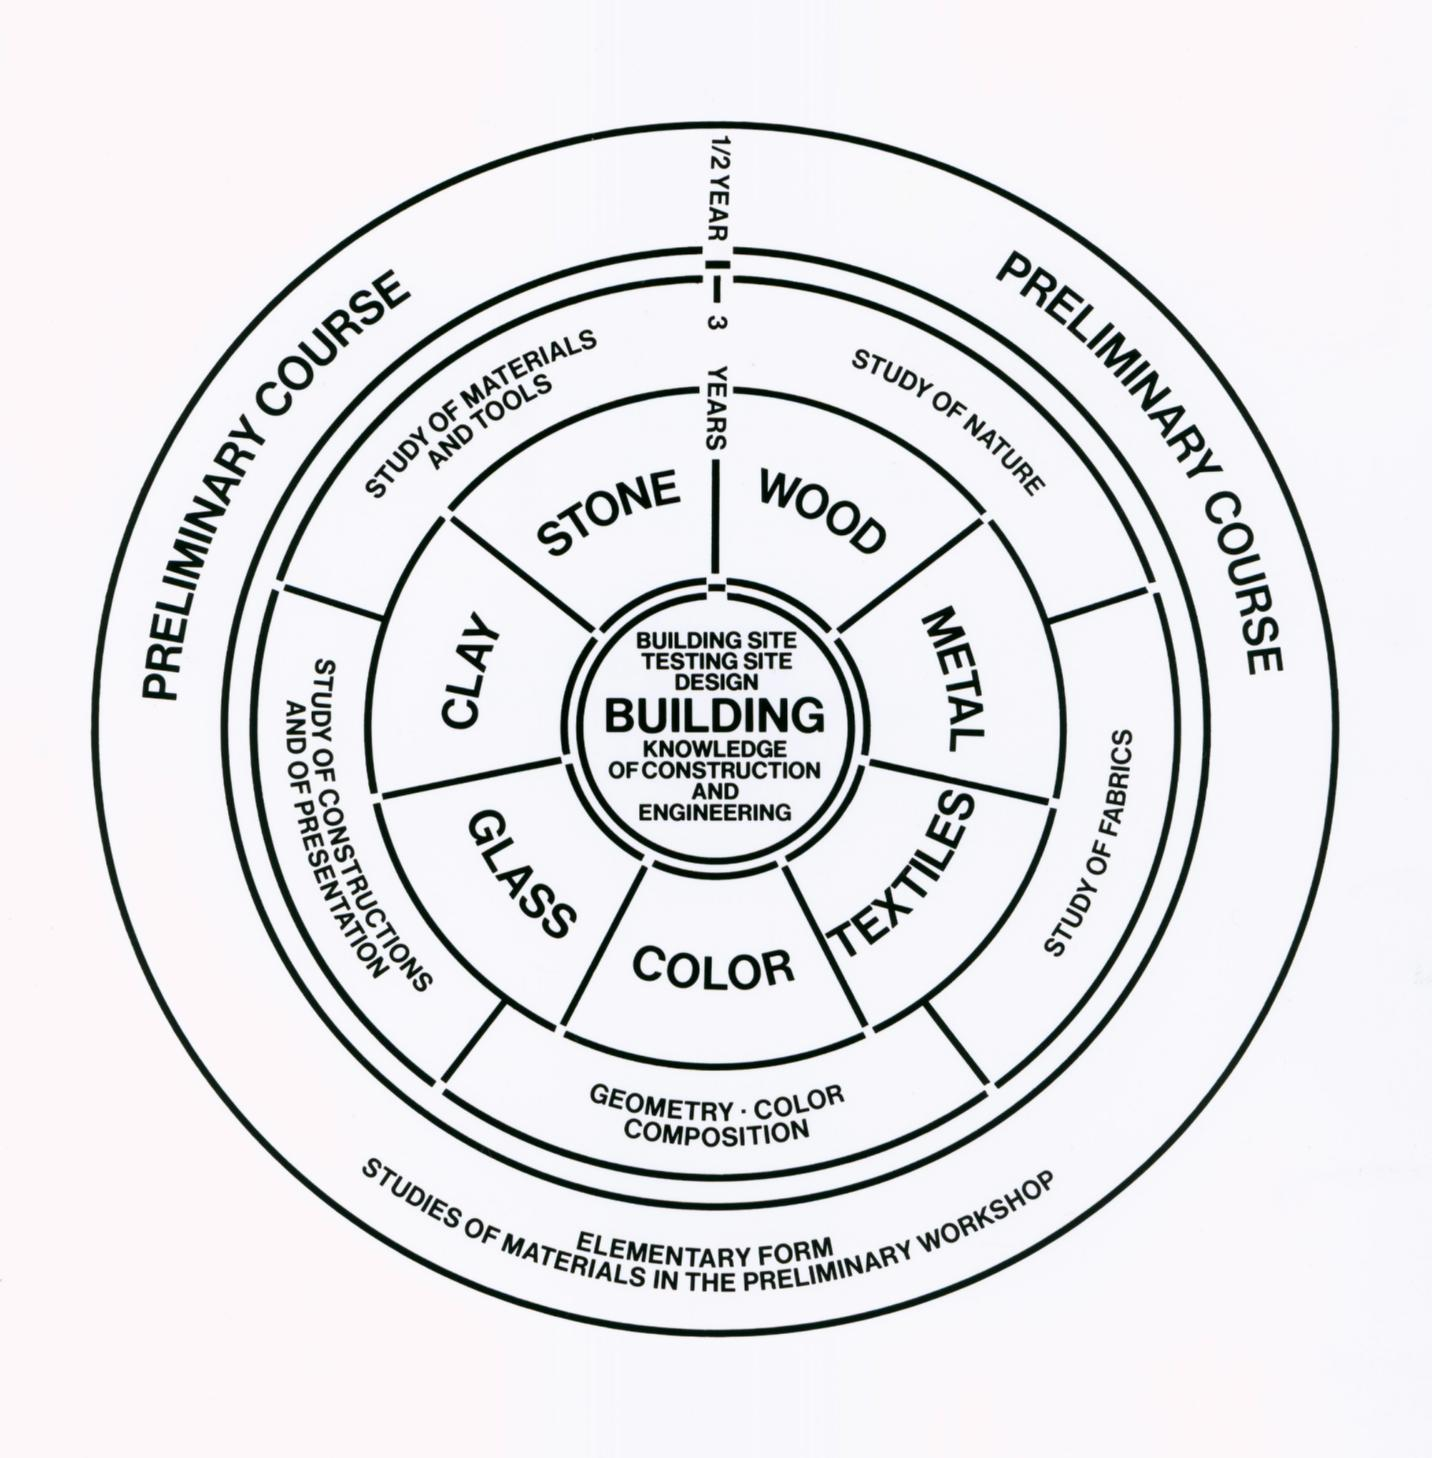
\includegraphics[width=1\textwidth]{pictures/bauhaus-curriculum-diagram}
 \caption{Diagram for the structure of teaching at the Bauhaus. Source: Walter Gropius, 1922.}
 \label{fig:bauhaus}
\end{figure}

\begin{figure}[h]
 \centering
 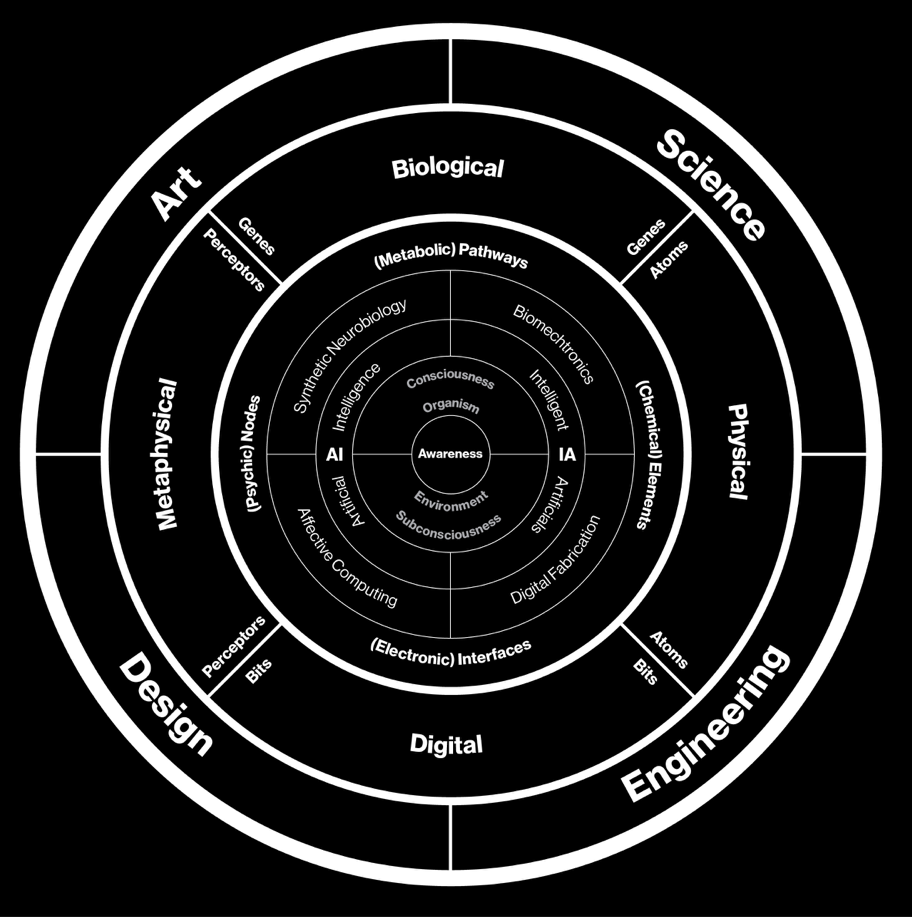
\includegraphics[width=1\textwidth]{pictures/krebs3}
 \caption{Krebs Cycle of Creativity III - Practice. Source: Neri Oxman, March 2018.}
 \label{fig:krebs3}
\end{figure}

\autoref{fig:bauhaus} is a diagram of the structure of teaching at Bauhaus in the 1920s. The Bauhaus brought together an interdisciplinary collection of disciplines, new materials and a new sensibility. In addition to a curriculum, the movement create a new style and form of architecture with real impact on the world.

Similarly, \autoref{fig:krebs3} is the third iteration of Neri Oxman's Krebs Cycle of Creativity. She is proposing a synthesis of disciplines, approaches and a sensibility that might be a way to create a new meta-discipline with a completely new way forward.

\marginpar{This inevitably requires challenging the institutions that have developed to support the academic process. We need to think about the structure of these institutions and how we might re-imagine them in the post-Internet era.} This inevitably requires challenging the institutions that have developed to support the academic process. We need to think about the structure of these institutions and how we might re-imagine them in the post-Internet era.


\subsection{Decentralization and Layers}
\label{decentralization}

The Internet, especially the early Internet, was a great example of the transformation of slow, powerful and incumbent institutions shown in figure \autoref{fig:monolith} into a vibrant and generative ecosystem.

Breaking up telecommunications' monolithic companies and monopolies required a new architecture of layers that unbundled the control at each layer. This allowed ecosystems of competitors and collaborators to form, decentralized control and innovation at the commercial layers, and creating an open and inclusive process at the protocol layers.

The Internet unbundled the layers technically and business-wise, allowing competition and innovation to flourish. This layering allowed the unbundling of power, interoperability, competition, and the highly generative Internet.

\begin{figure}[h]
 \centering
 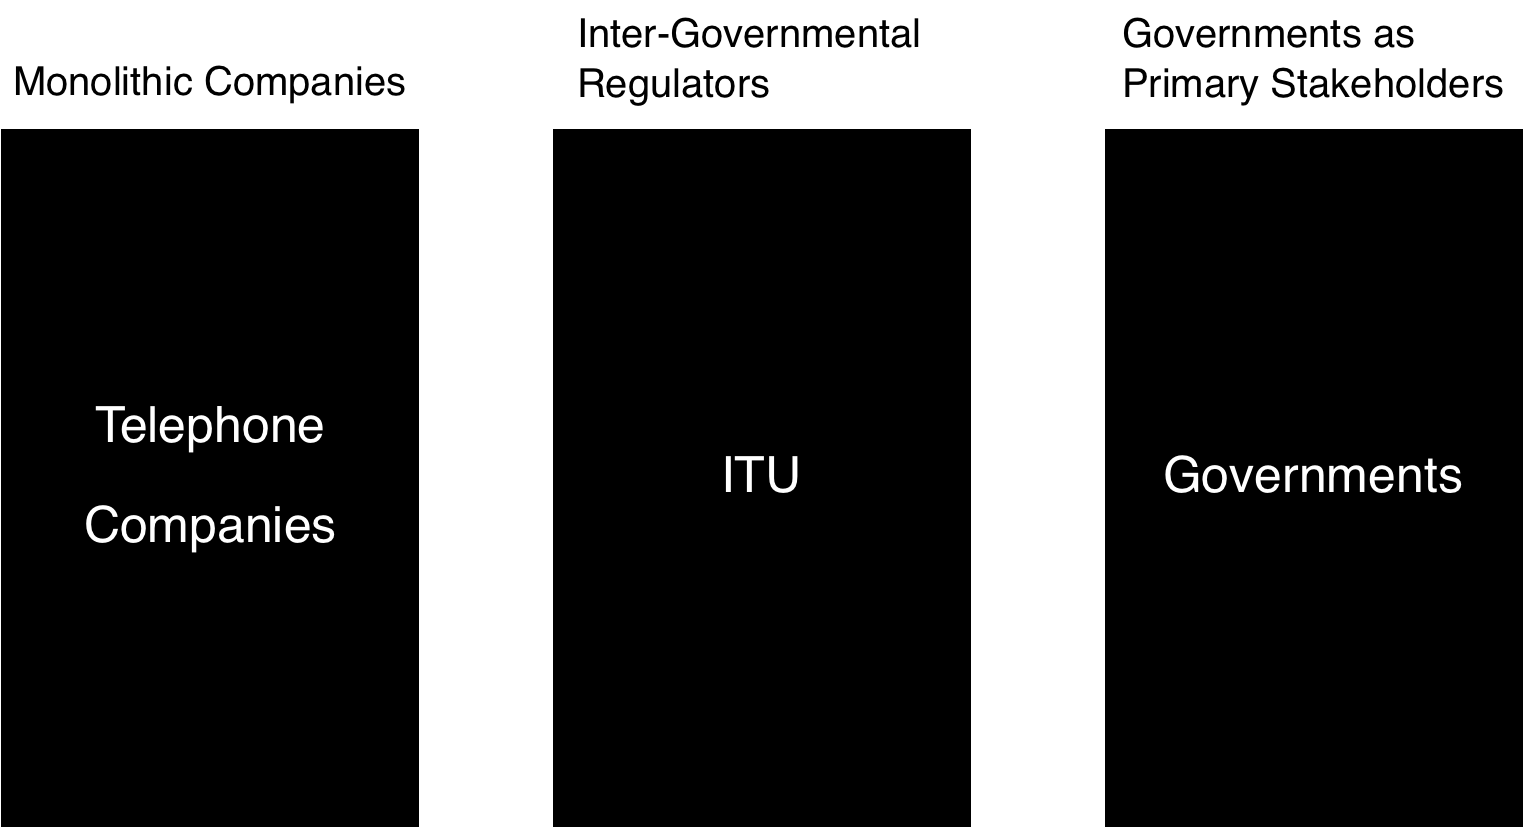
\includegraphics[width=1\textwidth]{pictures/monolith}
 \caption[Structure of telecommunications ecosystem before the Internet.]{Before the Internet, the telecommunications industry was monolithic telephone companies, working with inter-governmental regulators like the United Nations and the International Telecommunications Union and the governments themselves, creating a slow, bureaucratic, expensive, and closed system.}
 \label{fig:monolith}
\end{figure}

\begin{figure}[h]
 \centering
 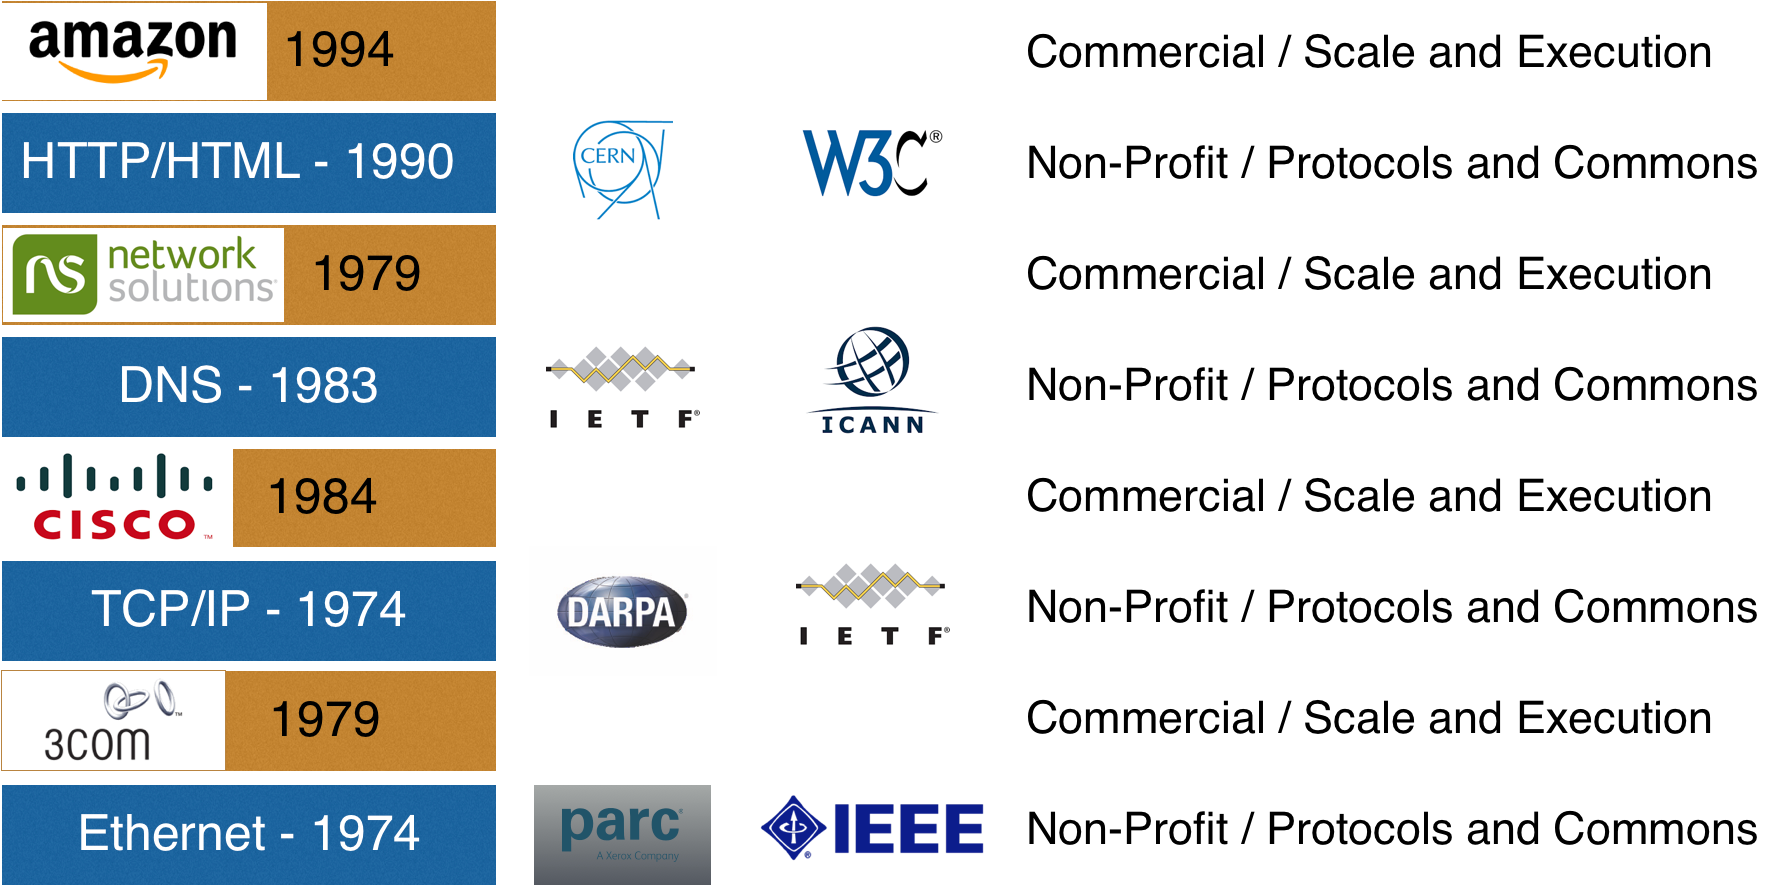
\includegraphics[width=1\textwidth]{pictures/InternetLayers}
\caption[Structure of telecommunications ecosystem after the Internet and its layers.]{The first column in this figure are the layers of open protocols and examples of companies creating the ``layer sandwich'' of the Internet. The next column is the funding or research organization that originated the protocol. The next column is the non-governmental not-for-profit standards body that currently stewards the protocol. The column on the right shows the role of that layer. The Internet unbundled the layers technically and business-wise allowing competition and innovation to flourish. Open Protocol and not-for-profit layers allowed communities of experts to design the best social and technical solutions without being encumbered by business and political interests. Commercial layers using these new open protocols were able to flourish and compete using the protocols to communicate with but be free from encumbrance from the layers above and below. This layering allowed unbundling of power, interoperability, competition and the highly generative Internet.}
\label{layertable}
\end{figure}

The personal computer and the Internet pioneered and perfected an architecture of unbundling the layers of a system --- chips, firmware, hardware, operating system, software, dark fiber and wire, modem, Ethernet, \ac{TCP/IP}, \ac{HTML}, website, browser. Each layer of the Internet (although PCs have similar layers) has an open protocol and standards stewarded by a non-governmental, not-for-profit organization with general but very clearly defined application programming interfaces, or \ac{API}s. Open protocol and not-for-profit layers allowed communities of experts to design the best social and technical solutions without being encumbered by business and political interests. Commercial layers using these new open protocols were able to flourish and compete using the protocols to communicate with, but be free from encumbrance from, the layers above and below. The system is decentralized. This architecture has significant advantages over monolithic systems in terms of efficiency and lower cost, resilience, interoperability of different technologies at each layer and the ability to continuously innovate rapidly.

\subsubsection{The Internet, Decentralization, Unbundling}

Before the Internet, telecommunications was centralized in monolithic telecommunications corporations. They controlled everything from pipes and wires to content. When multimedia first emerged, cable companies ran interactive video experiments and telephone companies like France Telecom and \ac{NTT} ran experiments such as Minitel and Captain.

The Internet was successful because we were able to unbundle its layers and create open and interoperable standards that allow companies to compete and create strong operational layers between open protocols. The key to open protocols was non-governmental coordinating organizations, such as \ac{ICANN} and \ac{IETF}. The \ac{API}s and protocols for communications between the layers was also essential.

The inventors of the protocols, such as Sir Tim Berners-Lee who created \ac{HTML} at \ac{CERN} and the team of academics who created \ac{TCP/IP} many years before, deliberately didn't patent their inventions. Instead, they established not-for-profit and non-governmental stewardship organizations to support a community of technical people and a process of coordination with stakeholders, as well as with similar \ac{NGO}s in other layers. They built interoperable systems that allowed systems and services to communicate with and build on top of each layer. These layers relied on consensus and were the essential ``commons'' of the Internet.

\marginpar{The primary risk, as we now see, is that while open protocols allow competition, they also allow companies to scalably harness the network effect \cite{web20} and we have seen monopolistic companies emerge in each of the commercial layers as a result.}It is notable that all of this original work was primarily academic and didn't involve governments except funding from \ac{DARPA} for early work in \ac{TCP/IP}. Government and traditional telecommunications attempts at creating something similar ended up in protocols such as \ac{X.25} that were complicated and encumbered by business and political interests that made them much less effective than the Internet protocol and lacked the fundamentally community-oriented and humble approach that made the Internet technical communities so generative and successful.

Built on top of these layers and between the ones above, the commercial layers of startups, mostly funded by venture capital, took open standards and scaled them and made them valuable and accessible to the public such as 3Com with Ethernet, Cisco with \ac{TCP/IP} and the browsers with \ac{HTML} (although Firefox is a notable not-for-profit example). For scaling and execution, for-profit, market-oriented ventures are extremely effective. The interoperable layers created a fertile platform for fair competition and disruption and allowed the emergence of companies such as Cisco on top of \ac{TCP/IP} and Amazon on top of \ac{HTML}. (See \autoref{layertable})

The primary risk, as we now see, is that while open protocols allow competition, they also allow companies to scalably harness the network effect \cite{web20} and we have seen monopolistic companies emerge in each of the commercial layers as a result. Nonetheless, so far even the biggest tech monopolies are eventually disrupted as technology advances, user behavior changes and new ventures come along to disrupt it --- Yahoo and Microsoft appeared to be indestructible monopolies until they weren't. However, Facebook and Google appear to be sustaining their stature so far.

Unbundling and interoperability has allowed the creation of a generative ecosystem that has thrived thanks to a kind of ``permissionless innovation.'' This was nurtured in great part by the diminishing cost of communication, collaboration and distribution, which helped sustain communities that generated the production of free and open source software. This greatly diminished the cost of innovation and pushed it out to the edges, into dorm rooms and to individuals who wanted nothing to do with large companies and traditional institutions.

I think unbundling and thinking of ecosystems in terms of layers linked by protocols controlled by open and inclusive nonprofit organizations is  applicable to many other vast systems including finance, virtual reality, international relations, government and artificial intelligence.

These organizations and communities can bring everyone together to coordinate the necessary relationship between government, markets, society and technology.

\subsection{Reinventing Health Care}
\label{theoryhealth}

\marginpar{As the Internet fundamentally changes the way that we see and interact with each other and the world, advances in artificial intelligence and machine learning are fundamentally changing how we understand and interact with health and medicine.}As the Internet fundamentally changes the way that we see and interact with each other and the world, advances in artificial intelligence and machine learning are fundamentally changing how we understand and interact with health and medicine.

To break through the impasse we have reached in determining the future of the pharmaceutical industry and to understand and develop diagnostic and therapeutic capabilities requires application of the antidisciplinary approach to the human body and health.

We must discover new inventions and paradigms to treat the diseases that we face, and create new tools. This requires abandoning the silos of disciplines and bringing all disciplines to bear on understanding health and designing a new structure for innovating to come up with solutions. To implement this vision, I have brought together mathematicians, physicists, systems biologists, computer scientists, new tools for visualizing and interrogating systems, and many others to try to get a better understanding of the science and how these systems work. We must question our basic assumptions and possibly invent new mathematics to model biological systems. We need to understand how to apply artificial intelligence and machine learning for understanding the systems, as well helping us create new diagnostic and therapeutic tools. In addition, the clinical trials for deploying new technology must be redesigned; using new tools such as machine learning and data science could significantly improve the way we test new methods. 

This cannot happen with the current structure of government funding and the discipline-segregated research university system. With the maturing of new technologies, the opportunity to evolve new paradigms for the future of health is here. We are already seeing signs of more streamlined processes; the ability to have new clinical endpoints, and greater insights into the patient experience via sensors. The application of such digital tools has generated data pools that have the potential to be explored via \ac{AI} and machine learning approaches. These new approaches will allow for a new development paradigm that will enable therapies and cures to be more targeted to individual patients and be delivered faster to market. For example:

\begin{enumerate}
\item In 2018, the 21st Century Cures Act was signed into law, a significant bipartisan legislative achievement aimed at accelerating the discovery, development and delivery of new cures and treatments. The Act issued an important directive to the FDA for the design and qualification of drug development tools, defined as biomarkers,  clinical outcome assessments, and any other method, material, or measure that is determined to aid drug development and regulatory reviews. It also advanced the idea of an ``information Commons'' for sharing data \cite{21centdatashare}. The law places heavy emphasis on leveraging innovation, advancing digital health technologies and developing next generation analytical approaches to improve health care, broaden access and advance public health goals. We are poised to enter an era of exponential growth of new machine learning, \ac{AI} and gene editing techniques for biological, preclinical and clinical research problems. Health and pharmaceutical companies could benefit vastly by using \ac{AI}-based generative, classification and prediction tasks to solve their most important challenges. Two specific examples of advanced analytics that could leapfrog the drug development process, in synergy with the Cures act, are listed below:

\begin{enumerate}
\item Complex systems-level datasets created from next-generation sequencing, transcriptomics, proteomics, metabolomics and single-cell experiments from patient samples and animal models can be processed with \ac{DNN} architectures.
\item High-throughput screens geared towards small-molecule discovery use manual processing, and in silico\footnote{\textit{In silico} is means ``performed on computer or via computer simulation.'' The phrase is an allusion to the Latin phrases \textit{in vivo}, \textit{in vitro}, and \textit{in situ}, which are commonly used in biology \cite{wikipedia:insilico}.} prediction of hits and potential targets and mechanisms. These tasks could be automated as new generative \ac{AI} systems can be used to design effective small molecule candidates.
\end{enumerate}
\end{enumerate}


\subsection{Lessigian Quadrants}
\label{sec:lessigq}

In his book, \emph{Code and Other Laws of Cyberspace} \cite{lessig2009code}, Lawrence Lessig describes four quadrants --- law, markets, norms and architecture (See \autoref{fig:lessigian}) --- as the four factors that influence what an individual can do. Architecture, in his definition, is the technical architecture, and he explains that laws can affect norms, markets and architecture. As an example he considers ways to get people to drive more slowly down a street. You could install speed bumps, a technical intervention, or you could establish a more stringent speed limit and enforce it, a legal intervention. You could also perhaps make it socially unacceptable to speed down the road, which would involve norms, or perhaps reward drivers financially for slowing down, a market solution. 

\begin{figure}[h]
 \centering
 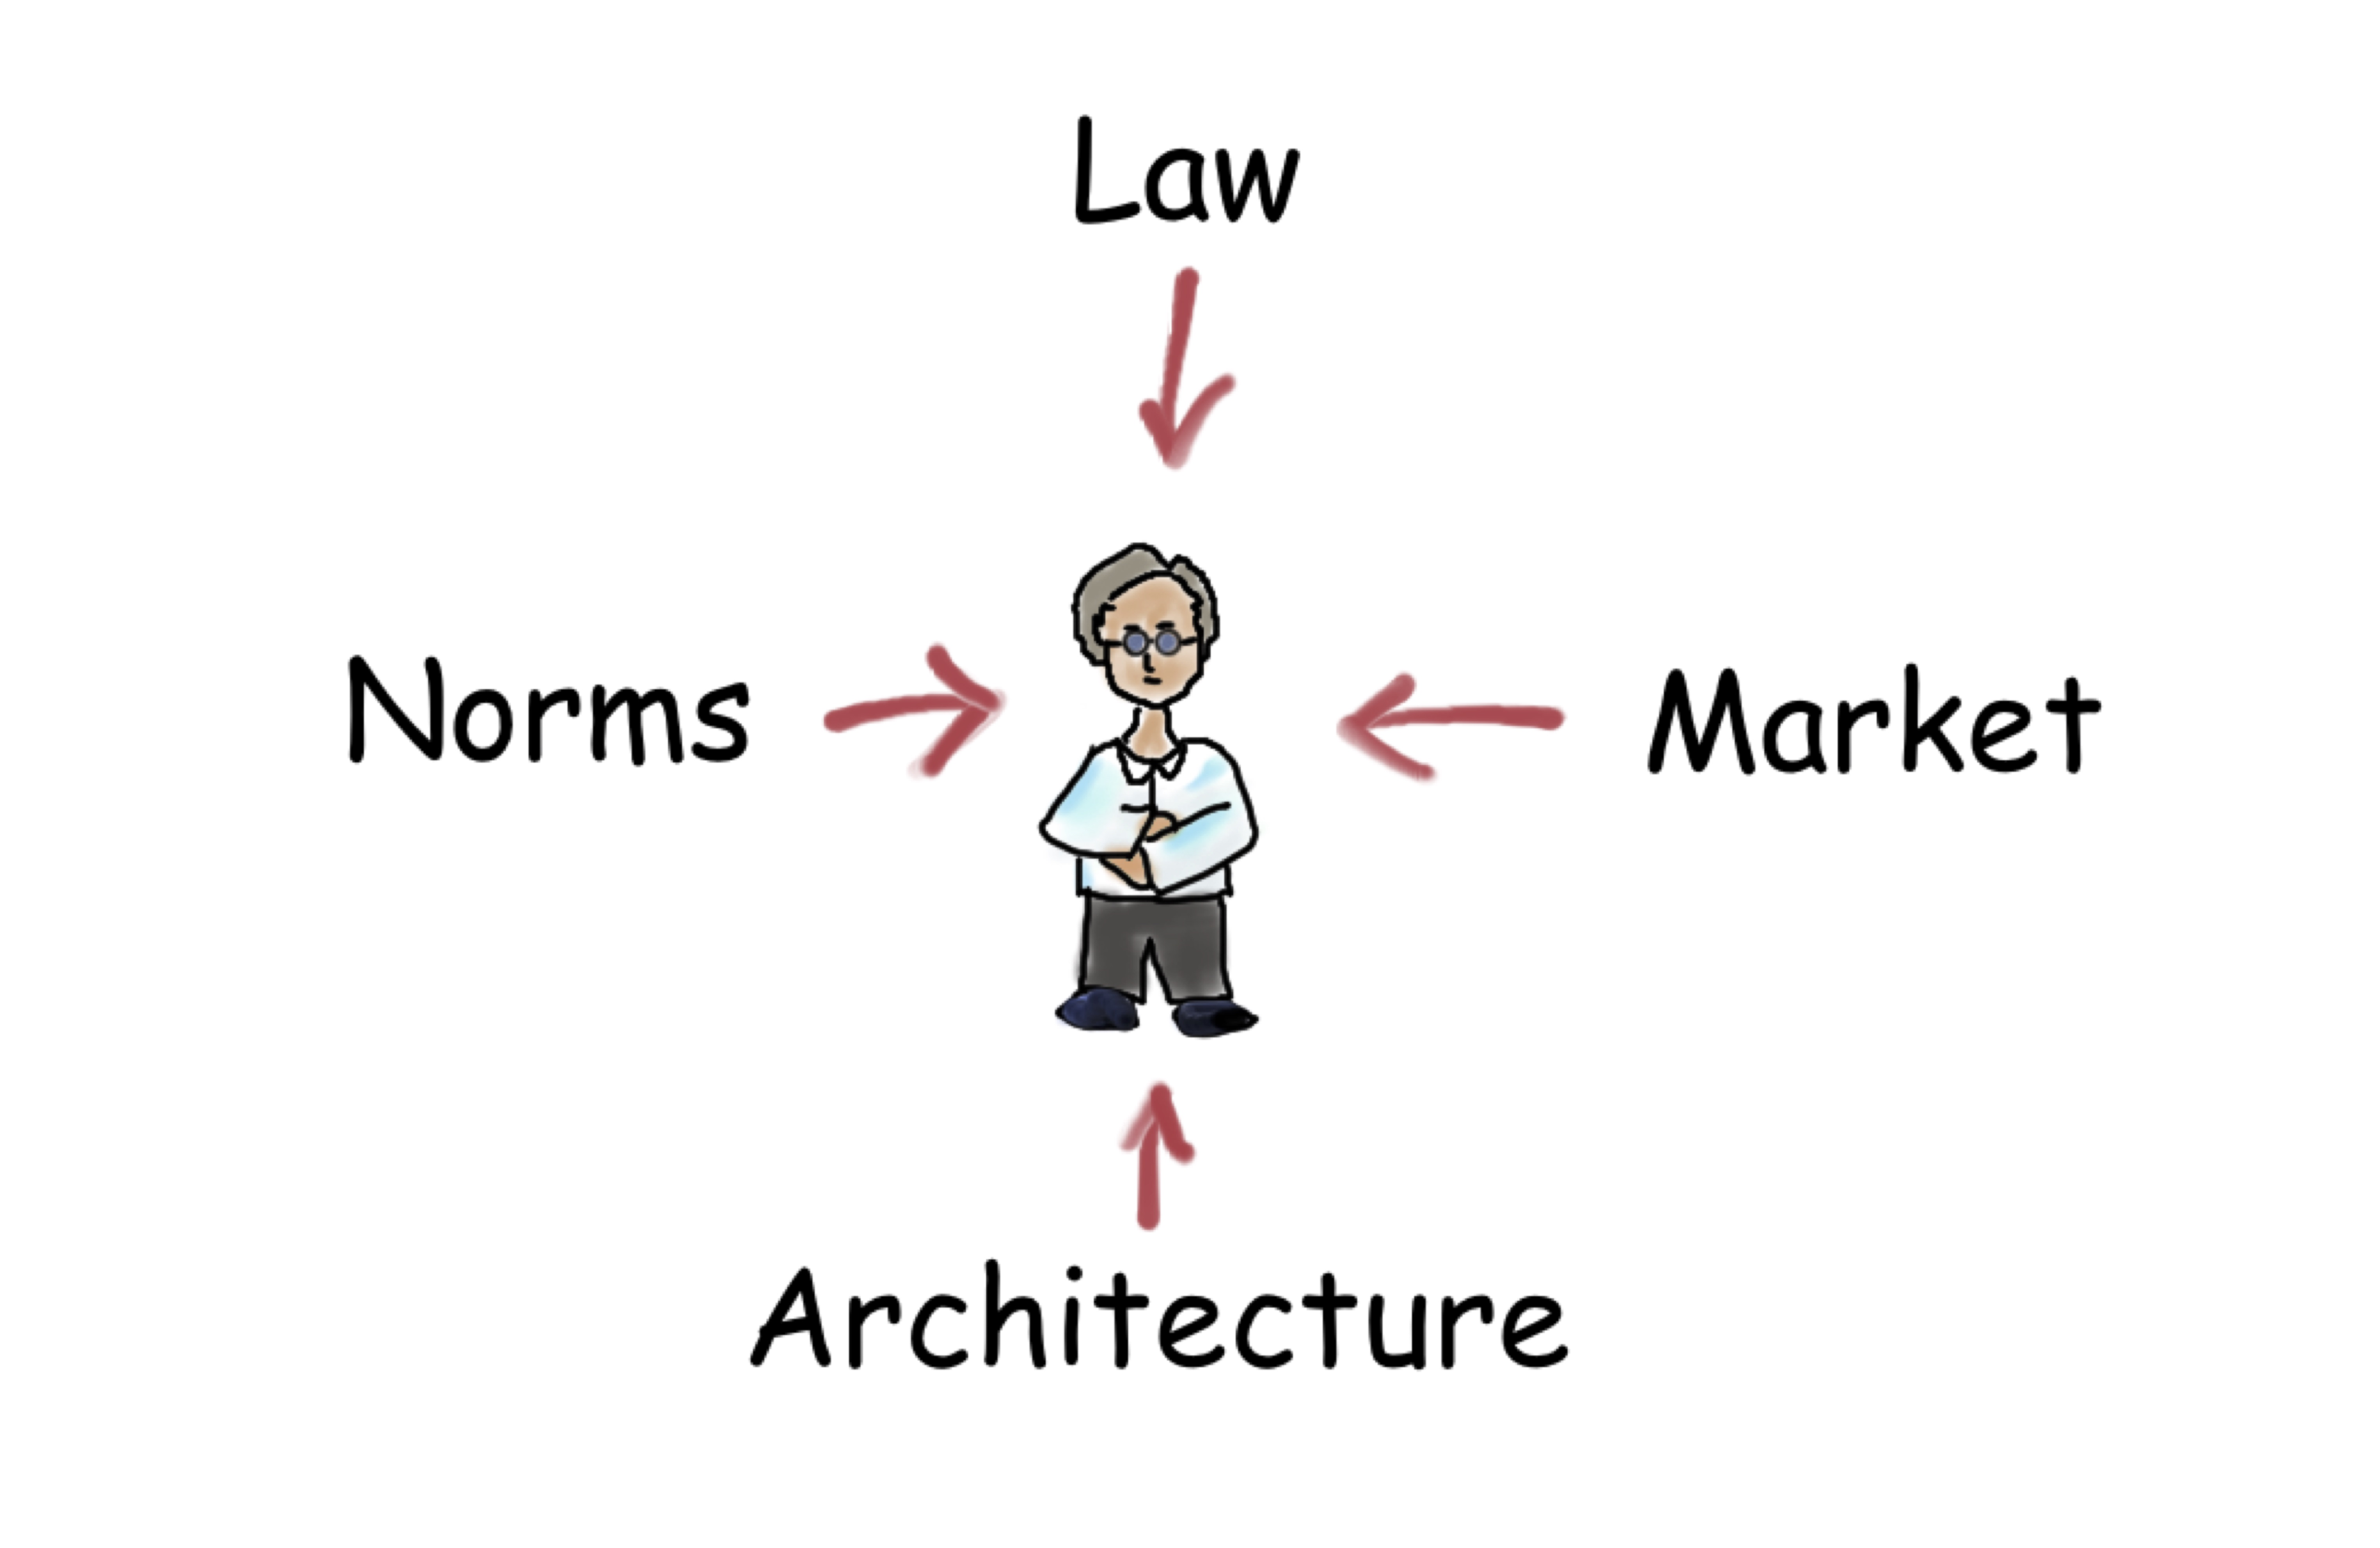
\includegraphics[width=.5\textwidth]{pictures/lessig.jpg}
 \caption{Lessig and the four quadrants. Image by Iyad Rahwan.}
 \label{fig:lessigian}
\end{figure}

One of the key points of Lessig's book is that a combined understanding of technical code and legal code became necessary for designing an appropriate legal and technical infrastructure once platforms such as the Internet emerged. For example, when the Internet made it possible to copy music and other copyrighted media, services such as Napster made it technically very easy to share music. Hollywood reacted by passing strict laws and enforcing them. This diminished the ability to share and remix creative works on the Internet. Eventually, Apple Inc. made a market intervention by building iTunes, which made the experience of sharing music legal and technically simple at a reasonable price --- and created a financial bonanza for itself by putting the company in an advantageous position in the market.

Around the same time, the record labels went after sampling, a key component of hip hop music. As they started suing artists who sampled, people stopped sampling as much. This changed the norms and in the US with common law, the norms changed the interpretation of the law. The norms of society were forever changed, and sampling music became illegal. Remix as a musical art form in the US was stopped dead in its tracks.

In other places, such as Brazil, things played out very differently. Markets and cultural norms actively promoted sharing, sampling and remixing, and focused on live performances to generate revenue. The event producers funded artists and the distributions of copies of the music were not policed \cite{shaver2010access}.

The upshot of Lessig's argument is that the four quadrants need to coordinate with each other, and incorporating all four quadrants at once is likely to yield the most effective and appropriate approaches to managing the development and deployment of technology in our society. This requires more than just a bit of interaction and negotiation between the quadrants, but rather an approach that goes beyond traditional disciplines --- an antidisciplinary approach.

\marginpar{Lessig's quadrants and an antidisciplinary approach are required for developing new rules as well as fixing broken ones.}Lessig's quadrants and an antidisciplinary approach are required for developing new rules as well as fixing broken ones.

%\subsection{Fixing Broken Protocols}
%
%As technologies change, many of the laws and regulations that made sense in the past, stop making sense. In the following essay from 2017, I describe a number of laws from money laundering to copyright to wiretapping and how the way in which they are broken is similar and how a Lessigian approach is necessary to fix them.
%
%\emph{Original title:
%\textbf{Why anti-money laundering laws and poorly-designed copyright laws are similar and should be revised}} \\
%
%\emph{Originally published October 13, 2017} \\
%
%\emph{Abstract: Intentionally or unintentionally, poorly crafted or outdated laws and technical standards threaten to undermine security, privacy and the viability of our most promising new technologies and networks, such as Bitcoin and the blockchain. We should vigilantly be reviewing and revising laws and standards for the public good and working to prevent the creation of fragile and cumbersome systems designed to comply with these poorly crafted or outdated laws. In this post, I discuss the Digital Millennium Copyright Act's Anti-Circumvention provision, Digital Rights Management, Anti-Money Laundering Law, Know Your Customer Laws and security backdoors.} \\
%
%The Internet's founding principles --- openness, unbundling, diversity, open standards --- made it robust, a force for democratizing access. That access created an explosion of innovation far beyond anyone's imagination.
%
%The Internet's openness is its strength. It is a ``stupid network'' \cite{isenberg1997rise} whose internals are unbundled into layers of open standards that sandwich layers of diversity and innovation. Stupid networks focus on transporting bits from one place to another. That end-to-end principle allows for innovation at the network's edges. By ``unbundling'' the transportation of bits from the provision of services, applications can be developed without permission. This is where we get the innovation in services that the network's architects and managers never imagined or had to plan for.
%
%There is a perennial call to ``make the network smart.'' Someone always wants to optimize it, establish ``quality of service'' mechanisms --- for example, to make voice calls more reliable. But whenever you optimize the network for one thing, you risk de-optimizing it for another. It turns out that just adding more bandwidth has been cheaper than making the network ``smarter.'' (This argument --- that you fix networks by making them faster, not smarter --- is key to understanding net neutrality.)
%
%Policy makers grapple with the nature of the open Internet with varying results. Sometimes they'll pass rules or orders that ``break'' these principles or induce changes in the Internet's architecture that work against its openness. These are usually the result of pressure from law enforcement or corporate capture in regulation and standards.
%
%Here are a few of the worst offenders: rules, laws and standards that do damage to the net's architecture, exceeding any benefit they deliver for their champions:
%
%\subsubsection{The Anti-Circumvention Provision in the Digital Millennium Copyright Act}
%
%Sections 1201-1203 of the 1998 Digital Millennium Copyright Act (DMCA) make it illegal to circumvent locks that restrict access to copyrighted works regardless of whether you are actually breaking copyright law. This means that companies can use digital locks to hide content to which we should have legitimate access, and those locks have the force of law --- breaking them is a felony with a maximum sentence of five years in prison and a \$500,000 fine.
%
%It doesn't matter how legitimate your access is. You could be delving into your own car's computers, your medical implant's data-streams, or even content you created on devices you own yourself. (Farmers who gather soil-density surveys of their own fields while driving their tractors around them are not allowed to see those data unless they buy the data back from John Deere). This also inhibits research that focuses on whether the security of such systems is robust.
%
%The FDA, for example, has been trying to get medical device companies to allow hacking currently prevented by the DMCA \cite{fda_2016}. The Library of Congress has added car software to the list of exemptions from anti-circumvention \cite{selyukh_soon_2015}, but unfortunately it appears that "exemptions created under the rulemaking apply only to the act of circumvention, and not the development and distribution of circumvention tools." \cite{noauthor_exemptions_2017} Tough luck for drivers and researchers who aren't also encryption experts.
%
%\subsubsection{Digital Rights Management (DRM) \& The World Wide Web Consortium (W3C)}
%
%The W3C is currently standardizing DRM for use in \ac{HTML}5, the next generation of core Web standards. By allowing DRM to be included in the standard, we ``break'' the architecture of the Internet by allowing companies to create places to store data and run code on your computer that you do not have access to and where breaking into code on your computer would constitute breaking the law. This is both a security risk and a fundamentally fragile system where vast amounts of content and information could be lost in the future as technologies evolve and companies change.
%
%While DRM has been touted as critical for business, it is clear that people are willing to pay for streaming and licensing of content without technical protections. If someone could actually afford to pay the fees currently charged by the streaming vendors, why would they go to an illegal pirating site to download something? Netflix, Apple Music, Spotify and Pandora would most likely not even notice, nor would their users, if they removed DRM technology. While it may not be in their interest to announce the death of DRM, it's likely to die a quiet death.
%
%In the meantime, we will be left with a broken and fragile architecture, as well as browsers whose internals are off-limits to security researchers, who face brutal punishment for trying to determine whether your gateway to the Internet is secure enough to rely on.
%
%\subsubsection{Anti-Money Laundering Law (AML) and Know Your Customer Laws (KYC)}
%
%There are many laws that have been created to prevent money laundering - crimes that disguise the original ownership and control of the proceeds of criminal conduct by making such proceeds appear to have derived from a legitimate source. One of the reasons these laws exist is to track terrorists and criminals by monitoring money flows.
%
%Laws to prevent money laundering create a requirement to report transactions above a threshold (usually \$10,000), to report assets held anywhere in the world in your tax returns and for banks to ``know your customer'' and keep detailed records of who their customers are and what they are doing. Breaking these regulatory requirements is illegal. Like the anti-circumvention law, while you may not actually be laundering money, breaking these anti-money laundering monitoring systems constitutes a crime.
%
%The personal information and transaction details are collected are stored in databases, and this presents a substantial risk to society. Criminal and foreign government hackers have over and over again hacked the most protected of government databases, such as the personal information of US government employees with security clearance in the OPM database \cite{nakashima2015hacks}. In addition, these laws require banks and financial institutions to collect this information and structure their systems to allow this information to be collected, also making these systems vulnerable to attack.
%
%While access to this information can sometimes be useful in investigations, almost all of the sophisticated technology to ``catch the bad guys'' doesn't require access to the content of the messages, but rather only access to the metadata. This is evident in modern Signal Intelligence (SIGINT: the collection of data ranging from satellite communication to Internet packets), where intelligence and law enforcement agencies rely mostly on machine learning (artificial intelligence) and pattern recognition extracted from metadata, rather than from the content of the messages. (Snowden released a document revealing the state of the art of goverment SIGINT \cite{noauthor_himr_2011}.
%
%We are already seeing both research and practice in conducting SIGINT on the blockchain \cite{spagnuolo2014bitiodine}. With Bitcoin and Blockchain technology in ``vanilla'' form, the ability to perform SIGINT is actually HIGHER than traditional more closed systems. AML and KYC laws are often impossible to implement while balancing the privacy of the users because the Blockchain is potentially visible to the whole world and not under the control of the selected entities. In fact, I believe that we must not only prevent the collection of the same kind of information in traditional financial system, but we must also discuss developing technologies to prevent privacy risks from the analysis of the Blockchain. If we are to deploy Blockchain broadly, we will have to look at both AML and KYC laws and upgrading them, taking into account the new technical architecture and environment and balancing the privacy and security concerns.
%
%The traditional financial system as we know it will undergo significant changes in the future, especially if we are headed in the direction of Bitcoin and Blockchain. We cannot expect the current AML and KYC laws to work in this new dimension: these laws were conceived for closed, highly guarded systems and not for international, open, technical standards. For instance, the ``travel'' rule \cite{noauthor_funds_2010} requires financial institutions to pass personal information to the next financial institution when transmitting funds. There is currently no secure or easy way to do this on the Blockchain.
%
%Just like with the Internet, weaknesses in networks like the Blockchain propagate to countries and regions where privacy risks to users could cause significant risks to human rights workers, journalists or anyone who questions authority. The conversation on creating new AML and KYC laws for new financial systems like Bitcoin and Blockchain needs to be a global one.
%
%\subsubsection{iPhone/Backdoors}
%
%While putting backdoors on all of our communications and/or banning encryption hasn't been passed as a law, there is a precedent for what is going on with Apple and the FBI. In the 90s, as telephones were going from analog phone lines to digital, the FBI argued that it could become more difficult to serve wiretap orders on phone companies. Rather than connecting alligator clips to wires at the phone company's offices, they would have request their own backdoor on the switches the phone companies used.
%
%When the government offered to pay the cost, the phone companies accepted the deal and the Communications Assistance for Law Enforcement Act (CALEA) was born. The FBI has built an extensive data collection system on top of this system. (One distinction is that CALEA is about backdoors on the transport platform, while the current iPhone debate is about encryption on the edges of the network.)
%
%While Silicon Valley appears to be resisting the government requests more than the telephone companies did, they are under constant pressure, and as the Snowden documents have revealed, it appears that many companies have provided these back doors.
%
%While I'm sure law enforcement officers would love to have even more tools for their investigations, we already have more tools to track and monitor the ``bad guys'' than at any time in history. The problem with backdoors is that they create a fragile infrastructure. So that even if you believe that we can trust the US government and US law enforcement, this creates a weakness that can be exploited by the ``bad guys.''
%
%One great example of the backdoor that was recently found on the Juniper's ScreenOS Software \cite{green2015juniper}. It appears that the government may have created a backdoor on a key secure communication channel, but that someone else (unknown), put a backback door on it exploiting the backdoor to make it their own.
%
%In my view, the risk to everyone on the Internet caused by crippling security isn't worth the incremental increase in the ability for any government to engage in legitimate surveillance. This point was made clear by the President's Review Group on Intelligence, an expert group, which said that the US government should ``fully support and not undermine efforts to create encryption standards; (2) make clear that it will not in any way subvert, undermine, weaken, or make vulnerable generally available commercial encryption'' \cite{abelson2015keys}. These are just some examples of the ``broken'' laws and standards. If we do not work actively to prevent the passage of bad laws and standards, and fight to overturn or fix the existing ones, we will soon lose the Internet and all of the freedoms, innovation and opportunities that it represents.
%
%Some of my colleagues and members of the Internet community seem to believe that we can ignore regulators, or that regulators are fundamentally at odds with our best interest. I believe that we can't ignore regulators because they will eventually pass laws that impact the scope and the way in which the technology we are developing is deployed. I also believe that many regulators do believe in trying to strike the right balance, and to engaging with the right people in the right context to help create technical standards and laws that actually work in the real world. We have had many successes such as a relatively unregulated early Internet, but we have also made some mistakes. For instance, were able to stop some mistakes like SOPA and PIPA \cite{noauthor_protests_2018} and also the Clipper Chip \cite{levy1994battle}, but many laws such as the anti-circumvention piece of the DMCA made it through.
%
%I believe that we need to vigilantly monitor the activity of lawmakers, regulators, standards bodies and industry groups and their activities. We must constantly review existing legal and regulatory frameworks as we develop new technologies to make sure that they make sense and not default to trying to apply existing laws and regulations to new technologies without careful review from first principles.
%
%One of the reasons I am involved in organizations such as Creative Commons and am excited about helping to create the Digital Currency Initiative at MIT is because I am interested in trying to avoid mistakes that could undermine the full potential of open and interoperable networks, such as the network of trust and value that Bitcoin and the Blockchain represent. I hope to play a role in working with all parties, such as the users, the technical community, businesses and regulators in trying to develop and implement sustainable and healthy ecosystems that will not ruin the technology or our freedoms, while providing appropriate safeguards and structures for civil society, business and government.

\subsection{Aesthetics of the Internet - Context as a Medium}
\label{userrise}

The Internet is a new technology, but it is also a platform and a medium. It is a kind of place. In ``Understanding media: The extensions of man'' Marshall McLuhan famously said, ``The medium is the message'' \cite{mcluhan1994understanding}. In order to understand what that means and how we most effectively work in the age of the Internet, we must explore what the Internet is as a medium.

Since the early 90s, I served as a jury member for the Prix Ars Electronica, one of the preeminent electronic art awards and conferences. The competition and the associated symposium provided artistic and aesthetic views on new technologies and help define these  as a medium for arts and designs. As a jury member for over a decade in the Internet category, I helped guide the development of Internet art by giving awards to interesting projects that seemed to capture the essence of the Internet. Schools and artists took cues from our awards and developed the field with us.

I was a member of the first jury that created the Internet category. This was just as the web was emerging. As with other categories of Ars Electronica, many of the early winners in the Internet category were not artists.

The early computer graphics juries awarded prizes to supercomputer visualizations. Similarly, we gave awards to Wikipedia, e-cash/e-gold, Neal Stephenson and Linux. We were sometimes criticized by the art community as giving awards to things that were not ``art'' but I defended our decisions --- artists, in my view, stretch the boundaries of a medium, used the tools in ways that the creators did not anticipate and helped society understand the medium and the future of the technology.

I believe that Ars Electronica and the artists it identified helped provide a critical view of the Internet as an art medium, and provided many insights into the risks and opportunities it presented. Ars Electronica continues to provide an important lens into thinking about the future of the Internet, science, and technology.

\begin{quote}
\emph{Aesthetics of the Internet--Context as a Medium}\footnote{This is an essay that I wrote for the Ars Electronica conference catalog in 1997 \cite{ito1997aesthetics} describing what I believed to be the essential nature of the Internet.} \\

For Ars Electronica - June 19, 1997 \\

The Internet connects computers, people, sensors, vehicles, telephones, and just about anything together in a global network which is fast and cheap. This interconnectedness is the context. Context represents the way and the timing in which nodes are connected together. If content were the noun part of information, then context would be the verb part.

New forms of media and communications tend to mimic its predecessors. Carl Malamud gives the example of early television where television shows often consisted of a radio announcer and a microphone on the screen. The Internet often has been called a method of online publishing or online broadcasting. Magazine publishers tell me that Internet advertising on a computer screen doesn't compare to an excellent full page ad in a magazine. Television producers often compare gritty Internet video to the power of a excellent television commercial. The Internet as a medium is not suited for the delivery of high volumes of the same information to many people. Currently,* the Internet connects everyone together at rather low bandwidth at low cost. The Internet delivers context, and it is of this that we should be building the future the Internet.

Much of the information in today's world and on the Internet expires very quickly. Fifteen minute old stock quotes become free, instant stock quotes costing money. Yesterday's newspapers are free on the Internet, but today's (or tomorrow's) can cost you money. It is a relationship with the newspaper and its reporters that is more important than the database of old articles. Your Netscape browser will expire in weeks. Stealing an old Netscape diskette at a computer shop makes very little sense. Rather than downloading lots of software, on the Internet people remember where to find what they need, or better yet, who to ask or where to search. It is information about information about information... Just as our monetary system has become very abstract, our currencies represent something that really has no physical reality, most information on the Internet is about context, rather than content. Instead of the hard data of yesteryear that could be bound in a book, stacked in a warehouse and distributed by trucks, the information on the Internet is about being connected LIVE and about being in the right place at the right time.

Communities on the Net consist of a group of people connected to each other in the form of discussions, games, or some other form of two-way connectedness. People invest time and energy into these communities and these communities evolve into a complex aggregate of relationships between people mediated by a technology and a context. It becomes a kind of place. These communities are influenced by the underlying technology, but grow far beyond the technology itself. The technology is a kind of genetic basis on which a new organism can grow, receiving input from its environment through its participants.

Artwork, writing and other forms of content which are often nearly static in the slow moving physical world can also become living things in the fluid, high-speed context of the Internet. An interesting idea or design can quickly become a popular item to be sampled, edited and redistributed. The artist can view their work, or their child, quickly develop in something quite different from what it was originally intended to be. The original artist is the parent, but unlike a child raised in complete isolation, work on the Internet is educated and formed, for better or for worse, into a product of its environment and society. Putting work on the Internet is more like giving birth than creating a static object.

Communities, multi-user games systems, markets, search engines and router configurations are all context oriented. The aesthetic of context is the design of such context-oriented systems which are outstanding in their nature. A good context-oriented system causes the network of living connections to converge, interact and grow. It adds value to the network and attracts users and connections.

The Internet is a self-organizing adaptive system. As John Casti from the Santa Fe Institute pointed out in his talk at the Ars Electronica Memesis symposium last year, one can understand completely the process in which a complex adaptive system works, but it is impossible to predict what it does. The Internet self-organizes itself in the very interesting area between total chaos and order. Eric Hughes has called it a working anarchy. When order is forced onto the Internet such as rigid protocols or singular ubiquitous operating systems, that layer becomes very brittle and as one learns in catastrophe theory, a shock to the system can cause a huge amount of damage. One virus or bug in the system could take the whole system down. The more inefficient and diverse nature of the current memetic/software pool allows the risk to be distributed. Many small earthquakes can help prevent a catastrophic earthquake. It is the inefficiency and the small errors that can help the Internet adapt and grow without imploding or exploding.

Ordered efficient systems are also very susceptible to fluctuation amplification. With feedback going in the wrong direction, small fluctuations in economy, politics, traffic or opinion can be amplified by the super-efficient network and explode or crash. Nature uses feedback systems that dampen such fluctuations in an elegant way to contain the energy and balance the systems. This non-linear balance is becoming exceedingly more important than to make the system faster or more efficient. This balance can also be explained as the aesthetic of the context.

\marginpar{It is the use, familiarity and reproduction that makes a meme powerful and proves its aesthetic quality. The Internet artist and the meme both work in the medium of context rather than content.}Nearly complete chaos can also be found on the Internet in the sheer number of disorganized pieces of content and people. Total chaos can also be made much more useful by adding just enough context to help group the content and people into useful communities and networks.

Therefore, I would conclude that both complete order and complete chaos offer very little information, value or energy. Systems that help order chaos or disorder order are useful. In addition, the way in which these systems cause this non-chaos/non-ordered system to manifest should retain or create as much energy as possible while keeping a feedback system that prevents it from amplifying into destruction or dampening into nothing. This requires a group of rules or memes that attracts energy in the form of people, content, traffic, money, etc. and organizes this content in a way that grows and adds value. It is almost a kind of memetic engineering.

The memetic engineer/Internet artist is interested in coming up with an idea, software protocol or image that grows and evolves on the Internet. It is more about creating life than about creating a non-living piece of art. The memetic engineer seeks to have the particular meme copied and replicated where traditional artists are protective of their work. It is the use, familiarity and reproduction that makes a meme powerful and proves its aesthetic quality. The Internet artist and the meme both work in the medium of context rather than content.
\end{quote}

\section{Deploying Change}
\subsection[Resisting Reduction]{Resisting Reduction\footnote{This section is based on an essay that I wrote for the \emph{Journal of Design and Science} \cite{ito_resisting_2017} which has since become a special issue with contributed responses and plans for a book from MIT Press.}}
\label{intro:resisting}

As the sun beats down on Earth, photosynthesis converts water, carbon dioxide and the sun's energy into oxygen and glucose. Photosynthesis is one of the many chemical and biological processes that transform one form of matter and energy into another. The molecules created through photosynthesis then are metabolized by other biological and chemical processes into yet other molecules. Scientists often call these molecules ``currencies'' because they represent a form of power that is transferred between cells and processes to mutual benefit, ``traded'' in effect. The biggest difference between these currencies and financial currencies is that there is no ``master currency'' or currency exchange. Rather, each currency is useful only in certain processes, and the ``market'' of these currencies drives the dynamics that are ``life.''

As certain currencies became abundant as an output of a successful process or organism, other organisms evolved to take that output and convert it into something else. Over billions of years, this is how the Earth's ecosystem has evolved, creating vast systems of metabolic pathways and forming highly complex self-regulating systems that, for example, stabilize our body temperatures or the temperature of the Earth, despite continuous fluctuations and changes among the individual elements at every scale from micro to macro. The output of one process becomes the input of another. Ultimately, everything interconnects.

We live in a civilization in which the primary currencies are money and power. The Internet's currency is attention \cite{goldhaber1997attention} which converts to both power and money through voice and advertising. More often than not, the goal is to accumulate power and money at the expense of society at large. This is a very simple and fragile system compared to the Earth's ecosystems, where myriads of ``currencies'' are exchanged among processes to create hugely complex systems of inputs and outputs with feedback systems that adapt and regulate stocks, flows and connections.

While humans have tried to build resilient systems through the engineering and design of advanced agricultural systems, supply chain and physical infrastructure, our systems lack the diversity and complexity of natural systems which make them so self-adaptive. The mono-parameter financial paradigms that set our goals and drive the evolution of society today have set us on a dangerous course that  the mathematician Norbert Wiener warned us about decades ago. The paradigm of a single master currency has driven many corporations and institutions to lose sight of their original missions. Values and complexity are focused more and more on prioritizing exponential financial growth, led by for-profit corporate entities that have gained autonomy, rights, power and nearly unregulated societal influence. The behavior of these entities is akin to cancers. Healthy cells regulate their growth and respond to their surroundings, even eliminating themselves if they wander into an organ where they don't belong. Cancerous cells, on the other hand, optimize for unconstrained growth and spread with disregard to their function or context, rather like our contemporary corporate world.

\subsection{Singularity}

Decades before the U.S. Supreme Court effectively ruled that companies had the same free speech rights as individuals, Norbert Wiener called organizations such as corporations ``machines of flesh and blood'' and automation ``machines of metal'' \cite{wiener1988human}. The new species of Silicon Valley mega companies, which engage in the machines of bits, are developed and run in great part by people who believe in a new religion, Singularity. The term ``singularity'' was coined by Vernor Vinge in 1993 \cite{vinge1993coming} and expanded by Ray Kurzweil in \textit{The Singularity is Near} in 2005 \cite{kurzweil2005singularity}. This new belief is not a fundamental change in the paradigm, but rather the natural evolution of the pursuit of exponential growth applied to modern computation and science. The asymptote of the exponential growth of computational power is artificial intelligence.

The notion of Singularity --- that \ac{AI} with its exponential growth will supersede humans and that everything we have done until now is insignificant --- is a religion created by people who have the experience of using computation to solve problems heretofore considered impossibly complex for machines \footnote{Singularity is closely related to transhumanism --- the idea that we will transcend our current human intelligence through biological and computation and attain immortality and super-intelligence. I recently wrote about transhumanism in my \textit{Wired} column \cite{ito2018transhuman}.}. They have found a perfect partner in digital computation, a knowable, controllable system of thinking and creating with a rapidly increasing ability to harness and process complexity and bestowing wealth and power on those who have mastered it. In Silicon Valley, the combination of group think and the financial success of this cult of technology has created a positive feedback system that has almost no capacity for regulating itself because it receives scant negative feedback. While many holding these beliefs would resist having them compared to a religion, instead arguing that their ideas are science- and evidence-based, those who embrace the Singularity engages in quite a bit of arm waving, and make leaps of faith based more on trajectories than ground-truths to explain their ultimate vision.

Singularitarians believe that the world is ``knowable'' and that computers will be able to process the messiness of the real world, just as computer scientists and Internet entrepreneurs have solved many other problems that were thought to be unsolvable by computers. To them, this wonderful tool, the computer, has worked so well for everything so far that it must continue to work for every challenge we throw at it, until we have transcended known limitations and ultimately achieve some sort of reality escape velocity. Artificial intelligence is already displacing humans in driving cars, diagnosing cancers and researching court documents. The idea is that \ac{AI} will continue this progress and eventually merge with human brains and become an all-seeing, all-powerful, super-intelligence. For true believers, computers will augment and extend our thoughts into a kind of ``amortality'' --- the idea that while one may still die, that death is not the result of the grim reaper of aging.

\marginpar{But if modern corporations are a precursor to our transcendence, the Singulatarian view that with more computing and bio-hacking we will somehow solve all of the world's problems or that the Singularity will save us seems hopelessly naive.}But if modern corporations are a precursor to our transcendence, the Singulatarian view that with more computing and bio-hacking we will somehow solve all of the world's problems or that the Singularity will save us seems hopelessly naive. As we dream of the day when we have enhanced brains and amortality and can think big, long thoughts, corporations already have a kind of ``amortality.'' They persist as long as they are solvent, and they are more than a sum of their parts --- arguably an amortal super-intelligence.

More computation does not make us more ``intelligent,'' only more computationally powerful.

For Singularity to have a positive outcome requires a belief that, given enough power, the system will somehow figure out how to regulate itself. The final outcome would be so complex that while we humans couldn't understand it, ``it'' would understand and ``solve'' itself. Some believe in something that looks a bit like the former Soviet Union's master planning but with full information and unlimited power, while others have a more sophisticated view of a distributed system. But at some level, all Singulatarians believe that with enough power and control, the world is ``tamable.'' Not all who believe in Singularity worship it as a positive transcendence bringing immortality and abundance, but they do believe that a judgment day is coming when all curves go vertical.

\begin{figure}[h]
 \centering
 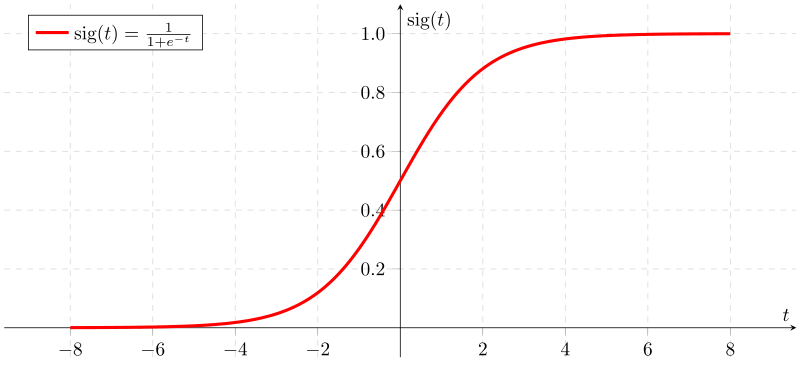
\includegraphics[width=1\textwidth]{pictures/Sigmoid-function}
 \caption{A Sigmoid curve otherwise known as an S-curve is defined by the formula $S(x) = \frac{1}{1 + e^{-x}} = \frac{e^{x}}{e^{x} + 1}$.}
 \label{fig:scurve}
\end{figure}

On an S-curve (see \autoref{fig:scurve}) or a bell curve, the beginning of the slope looks a lot like an exponential curve. In systems dynamics, an exponential curve shows self-reinforcement, i.e., a positive feedback curve without limits. Maybe this is what excites Singulatarians --- and scares systems people. Most people outside the Singularity bubble believe in S-curves, namely that nature adapts and self-regulates and that even pandemics will run their course. Pandemics may cause an extinction event, but growth will slow and humanity and society will adapt. But the notion of Singularity --- especially as some sort of savior  that will allow us to transcend the messy, mortal suffering of our human existence --- is fundamentally a flawed one.

This sort of reductionist thinking isn't new. When B. F. Skinner discovered the principle of reinforcement and was able to describe it \cite{skinner1938behavior}, we designed education around his theories. Scientists of learning know now that behaviorist approaches such as Skinner's only work for a narrow range of learning, yet many schools continue to rely on drill and practice. Take as another example the eugenics movement, which greatly and incorrectly over-simplified the role of genetics in society. This movement helped fuel the Nazi genocide by providing a reductionist scientific view that we could ``fix humanity'' by manually pushing natural selection. The echoes of the horrors of eugenics exist today, rendering almost any research effort to link genetics with things like intelligence taboo.

We should learn from our history of applying over-reductionist science to society and try, as Wiener says, to ``cease to kiss the whip that lashes us.'' While it is one of the key drivers of science --- to elegantly explain the complex and reduce confusion to understanding --- we must also remember what Albert Einstein said: ``It can scarcely be denied that the supreme goal of all theory is to make the irreducible basic elements as simple and as few as possible without having to surrender the adequate representation of a single datum of experience'' \cite{einstein1934method}. We need to embrace the unknowability --- the irreducibility --- of the real world that artists, biologists and those who work in the messy world of liberal arts and humanities are familiar with.

\subsection{Changing the Goals of a System}

\label{sec:meadows}

Donella Meadows described not only how systems worked, but how to intervene in these systems \cite{meadows_leverage}. By adjusting flows, feedback, goals, rules, how things are connected, etc., a system can be influenced and modified.

Meadows lists 12 ways to intervene in a system and lists them in reverse order of effectiveness.

\begin{quote}
\textbf{Places to intervene in a system according to Meadows}
(in increasing order of effectiveness)

\begin{etaremune} % downcounting enumerate
\item Constants, parameters, numbers (such as subsidies, taxes, standards).
\item The sizes of buffers and other stabilizing stocks, relative to their flows.
\item The structure of material stocks and flows (such as transport networks, population age structures).
\item The lengths of delays, relative to the rate of system change.
\item The strength of negative feedback loops, relative to the impacts they are trying to correct against.
\item The gain around driving positive feedback loops.
\item The structure of information flows (who does and does not have access to information).
\item The rules of the system (such as incentives, punishments, constraints).
\item The power to add, change, evolve, or self-organize system structure.
\item The goals of the system.
\item The mindset or paradigm out of which the system --- its goals, structure, rules, delays, parameters --- arises.
\item The power to transcend paradigms.
\end{etaremune}
\end{quote}

\begin{figure}[h]
 \centering
 
\includegraphics[width=.5\textwidth]{pictures/landlords-game.eps}
 \caption{The first patent drawing for Lizzie Magie's board game, \emph{The Landlord's Game}, dated January 5, 1904}
 \label{fig:landlords-game}
\end{figure}

The story of the game of monopoly provides a strong example of how these layers relate and why Meadows says the paradigm as the strongest driver of change in a system. Everyone knows the traditional Parker Brothers game of \emph{Monopoly}. What many people don't know is that \emph{Monopoly} \cite{monopoly} is based on a 1902 game called \emph{The Landlord's Game} \cite{landlords-game}, patented in 1904 by Elizabeth Magie (see \autoref{fig:landlords-game}). Magie's game was based on the economic principles of Georgism, which advocated a single tax on unimproved land, and the game was designed to show how rents enrich property owners and destroy tenants. Magie hoped that kids would play the game and learn about the unfairness of the capitalist system. The Parker Brothers version of the game didn't substantially change the rules --- it just changed the goal. Instead of aiming to teach children about the unfairness of capitalism, the goal of Monopoly was to become the capitalist and bankrupt all your friends. The thing to note here is that nothing in Meadows's list from 12-4 changed. Only the goal changed. As we think about how to ``fix'' the climate problem, by understanding that maybe somehow the goal --- to grow and eliminate the competition --- could change, maybe we don't need to change so many of the other layers. On the other hand, it might also show that even if we change a lot of the parameters and even the rules, unless we change the goal, we won't change much.

The goals are number three on the Meadows list. Number two is the paradigm --- in this case the paradigm of capitalism --- that drives the goal of what it means to win at the Parker Brothers version. The number one place to intervene is the power to transcend paradigms --- culture changes and paradigm shifts.

Goals and behavior are hard to change. We often believe that if we just labeled food better or if we could just make a convincing argument that our behavior negatively impacts the health of the planet, people would behave differently. But for many people, it's not an information problem. The Heart Attack Grill \cite{heart-attack} in Las Vegas serves Triple Bypass Burgers that have 9,982 calories and even Coronary Dogs. The waitresses are dressed as nurses and you eat for free if you weigh over 350 pounds. (see \cref{fig:heart-attack}) You often have to wait in line to get in, and several people have had heart attacks while eating there. In the case of the Heart Attack Grill, it's clearly not an information problem --- it's a culture, story and style problem.

\begin{figure}[h]
 \centering
 
\includegraphics[width=.5\textwidth]{pictures/heart-attack.eps}
 \caption{Heart Attack Grill}
 \label{fig:heart-attack}
\end{figure}


In 2008, Canadian health workers on assignment in Cambodia were trying to solve a health problem caused by a lack of iron in the diet of Cambodians. The workers tried handing out supplements and educating people about the need for iron, but none of that worked. They happened to hear a local story about a ``good luck'' fish. So they fashioned a fish out of iron that Cambodians could throw in their pots when they were cooking. The ``lucky iron fish'' was a huge success, delivering a significant positive health outcome \cite{charles2010iron}.

\subsection{Interventions through Arts}

Health workers are not the only people who try to modify behavior through cultural intervention. During the Cold War, the \ac{CIA} used modern art as a ``weapon'' to combat communism \cite{cia-communism}. The spy agency promoted modern art, which embodid the creativity and freedom that Russian art, tied as it was to communist ideology, lacked.

Intervening at the paradigm level of complex systems can be achieved by developing a sensibility appropriate to the environment and the time. These interventions are more like music than an algorithm. Music is about a sensibility or ``taste,'' with many elements coming together into a kind of emergent order. Instrumentation can nudge or cause the system to adapt or move in an unpredictable and unprogrammed manner, while still making sense and holding together. Using music itself as an intervention is not a new idea; in 1732, Andrew Fletcher (see \autoref{fig:fletcher}), a Scottish writer and politician, wrote, ``if a man were permitted to make all the ballads, he need not care who should make the laws of a nation'' \cite{brown2015eighteenth}.

\begin{figure}[h]
 \centering
 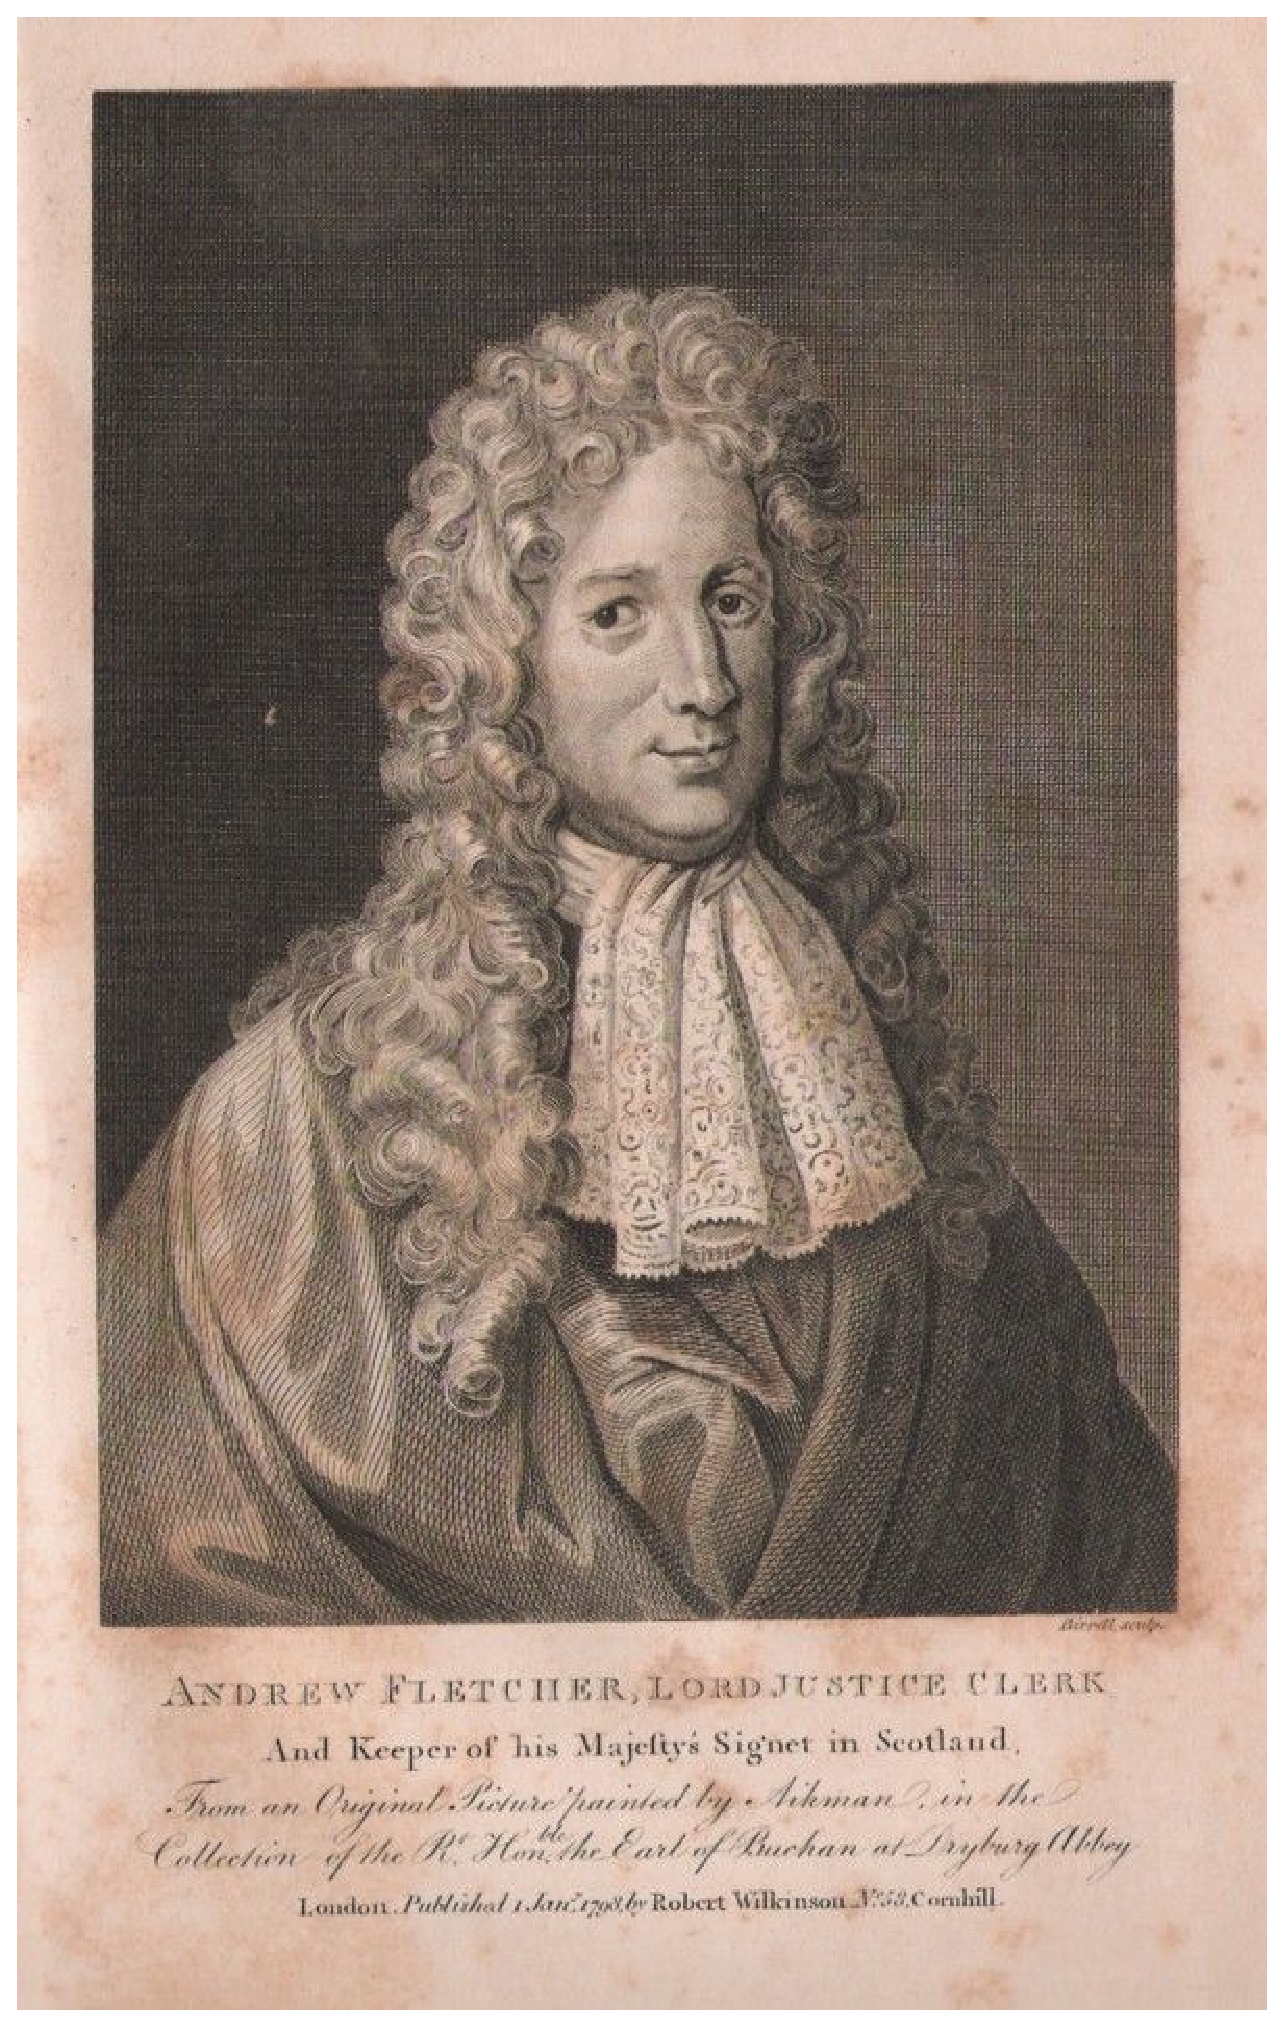
\includegraphics[width=.5\textwidth]{pictures/fletcher.eps}
 \caption{Andrew Fletcher of Saltoun (1655 -- September 1716)}
 \label{fig:fletcher}
\end{figure}

If writing songs instead of laws feels frivolous, remember that songs typically last longer than laws; have played key roles in various hard and soft revolutions,; and end up being transmitted person-to-person along with the values they carry. It's not about music or code. It's about trying to affect change by operating at the level songs do. This is articulated by Meadows, among others, in her book \textit{Thinking in Systems} \cite{meadows2008thinking}.

\subsection{A Culture of Flourishing}
\label{sec:cultureflourish}

Developing a sensibility and a culture of flourishing, and embracing diverse measures of ``success,'' depend less on the accumulation of power and resources and more on the variety and richness of experience. This is the paradigm shift that we need, and it will provide us with a wealth of technological and cultural patterns to draw from to create a highly adaptable society. This diversity also will allow elements of the system to feed each other without the exploitation and extraction ethos created by a monoculture with a single currency. It is likely that this new culture will spread as music, fashion and other forms of art as well as through spirituality.

As a native Japanese, I was heartened by a group of junior high school students I spoke to in Japan recently who, when challenged about what we should do about the environment, asked questions about the meaning of happiness and the role of humans in nature. I am likewise heartened to see many of my students at the MIT Media Lab and in the Principles of Awareness class that I co-teach with the Venerable Tenzin Priyadarshi using a variety of metrics (currencies) to measure their own success and determine meaning and grappling directly with the complexity of finding one's place in our complex world.

\marginpar{I think that it will yet again be about the music and the arts of the young people reflecting and amplifying a new sensibility: a turn away from greed to a world where ``more than enough is too much,'' and where we can flourish in harmony with Nature, rather than through control of it.}I'm also working with organizations such as the IEEE, which is designing guidelines for the development of artificial intelligence based on human wellbeing instead of simply around economic impact \cite{chatila2017ieee}. The work by Peter Seligman, Christopher Filardi, and Margarita Mora from Nia Tero \cite{NiaTero71:online} (described later in \autoref{sec:indigenous}) approaches conservation by supporting the flourishing of indigenous people, not undermining it. Another example is that of the Shinto priests at Ise Shrine, who have been planting and rebuilding the shrine every twenty years for the last 1,300 years, physically demonstrating the beauty and amazing capacity for renewal that we see in the cycle of nature.

In the 1960s and '70s, the hippie movement tried to pull together a ``whole earth'' movement, but then the world swung back toward the consumer and consumption culture of today. I hope and believe that a new awakening will happen and that a new sensibility will cause a nonlinear change in our behavior through a cultural transformation. While we can and should continue to work at every layer of the system to create a more resilient world, I believe the cultural layer is the layer with the most potential for a fundamental turn away from the self-destructive path that we are currently on. I think that it will yet again be about the music and the arts of the young people reflecting and amplifying a new sensibility: a turn away from greed to a world where ``more than enough is too much,'' and where we can flourish in harmony with Nature, rather than through control of it.


\subsection{Communities and Values}
\label{intro:communityvalues}

Meadows, in her essay ``Leverage Points'' \cite{meadows_leverage} about ``Places to Intervene in a System,'' explains that the most effective way to intervene in a complex system --- ``a corporation, an economy, a living body, a city, an ecosystem'' --- is with the power to transcend paradigms. That, she says, allows us to change ``The mindset or paradigm out of which the system --- its goals, structure, rules, delays, parameters --- arises.'' The goals determine the evolutionary direction as well as the direction of a system such as a community.

\marginpar{In ``Supercooperators: Altruism, evolution, and why we need each other to succeed'' \cite{nowak2011supercooperators} Nowak and Highfield describe the evolution of cooperation and mechanisms for cooperation. They argue that evolution is not only competition but also cooperation, and that cooperation is the master architect of complexity.}In ``Supercooperators: Altruism, evolution, and why we need each other to succeed'' \cite{nowak2011supercooperators} Nowak and Highfield describe the evolution of cooperation and mechanisms for cooperation. They argue that evolution is not only competition but also cooperation, and that cooperation is the master architect of complexity. In ``Spontaneous giving and calculated greed,'' researchers argue that people are intuitively cooperative and thus need to``calculate'' to overcome their cooperative impulse and become greedy \cite{rand2012spontaneous}. In ``Cooperating with the future'' \cite{hauser2014cooperating} the argument is that a large altruistic, majority would vote to cooperate with a longer view of the future in a democratic setting.


In Eric Raymond's 2001 classic, ``The Cathedral and the Bazaar: Musings on Linux and Open Source by an Accidental Revolutionary '' \cite{raymond_cathedral_2001} he describes traditional software development as the equivalent of a cathedral with top-down control and organization whereas open source software was more like a bazaar --- self-organizing and decentralized in nature. In ``Coase's Penguin, or, Linux and The Nature of the Firm'' \cite{benkler_coases_2002}, Yochai Benkler, a professor at the Harvard Law School, describes open source communities and introduces the notion of commons-based peer production. The firm, according to Ronald Coase, when he was a professor of economics at the University of Chicago Law School, increases productivity beyond gains that would take place simply in a free market by allowing the management of and the direction of resources in an organized way \cite{coase_nature_1937}. Benkler argues that the Internet has created  a way for participants in an open source project like Linux or Wikipedia to deploy their own labor to the tasks most suited to them without centralized management. He argues that because of lower costs and the decentralized nature of these systems, a community can be productive and create assets such as Linux and Wikipedia in the ``commons,''  outside of formal legal structures such as a firm or corporation.

The productivity of a community and what it produces is tied to how the community is designed and how well it is flourishing. Communities with productive outputs exist in many fields. For instance, communities of engineers work on open standards; communities of venture capitalists and entrepreneurs build startups in a startup ecosystem; communities of lawyers work on open source licenses; a community of developers work on Bitcoin; the community of members in a subculture like the hippie movement produced cultural products. It is the title of David Weinberger's 2002 book about the Internet, \textit{Small Pieces Loosely Joined} \cite{weinberger2008small}.

A flourishing community is very similar to a flourishing ecosystem with similar drivers, attributes and outputs. Turning back to Meadows' work on intervening in complex systems such as ecosystems, we can apply systems dynamics to communities as well.

As complex adaptive systems, communities can be resilient, they can collapse, they can grow, they can change. The values or paradigms of a community determine the aesthetic style of the output. The hippie movement embraced a world view that was natural, anti-establishment, psychedelic, loving and peaceful. Hippies wore tie-dye shirts, smiley face pins and long hair in solidarity with Native Americans, and their music was participatory and inclusive, producing musicians like the Grateful Dead. This sensibility also determined the evolutionary process that produced the movement's strategies and popular ideas, such as protests, communes and the emergence of the \emph{Whole Earth Catalog}.

The values of modern, neoliberal capitalism are fundamentally rooted in the paradigm of productivity and money, with almost everything measured in financial terms. Progress and growth of the economy are a kind of true north compass heading toward which everything is pointed, and it is against this payout that corporations, individuals and governments are measured and optimized. We have social services, culture, education and research, of course, but economic impact is the primary measure of their success and value. Established economists have questioned free market economics, from Economics Nobel Prize winner Elinor Ostrom's on sharing resources and governing the commons \cite{ostrom2015governing} to another Nobelist, Joseph Stiglitz, who criticizes free market fundamentalists and GDP as a reductionist measure of a healthy society \cite{stiglitz2010freefall}. However, their views have failed to sway the mainstream economic policies and behavior of society.

This has not necessarily been the case historically. Indigenous cultures such as Shinto, Maori, Native American, and just about any long-lasting historical community connected with nature typically have cultures based on flourishing together with nature and living in a vibrant but sustainable way. These values generate an internally coherent and rich culture with rituals, production and resilience that is nearly incomprehensible to those who live in capitalist, industrial cultures \cite{kohn2013forests}.

For instance, Shinto priests at Ise Shrine, as mentioned, have been planting and rebuilding the shrine every twenty years for the last 1300 years in a celebration of renewal and the cyclical quality of nature. The process involves many rituals, including fertilizing the mountains with oysters from the sea. For thousands of years, the shrine and its keepers have lived with and celebrated nature, not growing or ``improving'' but nonetheless flourishing. In fact, the seventh-century Emperor Tenmu banned livestock and meat, essentially establishing vegetarianism by fiat on an island that could not easily sustain a livestock-based food culture. Such values come from the nature-friendly, animist Shinto worldview \cite{zenjiro}. (Buddhist values also had a substantial influence.)

There have always been subcultures in society that have operated with alternative paradigms and goals. Some of these were different forms of governance with some of the same paradigms, such as communism with its  philosophy of managing resources and growing economies.

Other subcultures, such as hippies, developed new paradigms that transcended some of the basic paradigms of American society, with its worship of growth and the focus on property ownership. These movements and the communities that have supported them have played an essential role in the development of the Internet and positive social change, such as the civil rights movement. The next section will describe the role that the hippies and the Internet have played.

Many such sub-cultures and communities start through some sort of mind-expanding experience. Historically, these have come from contemplative practices that have driven religions like the Sufi, Gnostics, Yoga, Kabbalah and Buddhist meditation. These practices have often led to religious or spiritual movements that, at least at the beginning, seem to transcend the paradigms of the day, creating an alternative system, or sometimes co-existing, within traditional society --- church and state.

These cultures and subcultures are dynamic, merging, forking, dying, giving birth, cross-pollinating and so on. Some evolution in these communities is natural, but some of the change is a result of designers who have intervened in these systems by transcending paradigms, nudging values, making connectionsm and otherwise perturbing these communities.

In \textit{Social Physics}, Alexander Pentland, a faculty member at the Media Lab, describes the use mathematical models and data science to understand the flow of ideas through systems and how people react to them \cite{pentland2015social}. Using these new tools, we may make headway in understanding the spread and impact of culture and new ideas.

Evolutionary dynamics show that individuals use mutation to try new strategies, competing with each other for the payout. The most successful strategies reproduce and disseminate themselves. A system of different individuals cooperating and competing with each other creates an ecosystem. We can model a community as a kind of ecosystem with a competition of ideas, strategies and tastes that are determined to be more ``fit'' based on how they measure against the values of the community --- the paradigm. By influencing the paradigm, the community's evolutionary dynamics can be influenced. These dynamics can increase robustness and allow a community to adapt to changes in the environment or its relationship to other communities and intersecting systems at other scales such as health, the environment, or the technological.

They key method of my theory of change is to shift the paradigms in all of the systems described in this chapter by intervening in communities to influence their values and culture. That way we can change the evolutionary game that the individuals and the system respond to, and fundamentally change the behavior of the system and its outputs, structure, and growth. In this section, I explore learnings and different ways that we can intervene in, manage, and harness the power of communities.

\subsection{How Nightclubs Work}

While I learned a great deal from online communities, my early experience in the nightclub scene helped to provide me with some insights into how culture manages communities and communities manage culture in a much more visceral way.

When I was attending the University of Chicago, I started exploring the nightclub scene in the city. It was in the late 1980s when \ac{AIDS} was taking a huge toll, especially in the gay community. My fellow students were all fairly similar, relatively privileged and focused mostly on completing their degrees and getting a job.

What I encountered in the nightclubs in Chicago was a diverse community of working-class people helping each other, loving, sharing, supporting, and creating very humane and sophisticated systems to flourish in a difficult environment.

The nightclubs were a community but also the hub of many of different communities. I started spending a lot of time in a community centered in the North Side of Chicago, around the Cabaret Metro and the Smart Bar. I occasionally worked as a DJ at the Smart Bar. (I had a more regular DJ job at another club called The Limelight, but the community around it wasn't as interesting to me.) I learned a lot at the nightclub, and one of my most important learnings was that elite people in society often underestimated the values, intelligence, and contributions of working-class people. I also learned a lot about participating in and managing diverse and generative communities. 

A key learning was that influence in one community didn't necessarily translate into influence in another. Being rich, smart or famous in the ``outside world'' didn't translate to influence many other communities. Indeed, an effort to try to translate that influence often had reverse effect. It was also clear that these communities all interacted and that the complex set of relationships, values, and measures of influence created an extremely complex and resilient network quite incomprehensible from the outside.

A DJ in a nightclub has the ability to influence a very important currency in the physical space --- the music. This way a key factor in the behavior of individuals as well as groups in the space and that significantly affected the financial and social success of a nightclub. By changing the music, you can move different groups of people onto the dance floor, to the bar, out of the club, or get groups to mix with each other. Different songs or genres are familiar to different cultures and communities. Some songs make people dance, some make them stop and get a drink and some make them leave.

\marginpar{ The DJ is just selecting the ``background music'' but might have the most power to shape the culture of a club.}In addition, a DJ over time can lead the community around the club in new directions by introducing new trends in the context of the trends that the members of the community already know. The DJ is just selecting the ``background music'' but might have the most power to shape the culture of a club.

I eventually dropped out of the University of Chicago to become a professional DJ for awhile. I later moved to Tokyo where I ran a nightclub for a year to try to understand the cultural differences. I often think of being a DJ as a metaphor for what I do at the Media Lab and in other communities that I am part of: I watch the behavior and dynamics of the community and intervene culturally through music or equivalent higher level sensibilities to try to tune the flourishing and the direction of the community. This cannot be accomplished without a deep understanding of the relationships of the different subcultures, their tastes and the experiences and values that drive those tastes.



\subsection{The Hippie Movement}

The hippie movement was a movement with music as a key component among a rich array of elements.

The history of the hippie movement is well documented and has a number of interwoven narratives. Most will trace its roots to the legal and academic, at least initially, to the study and use of psychedelic drugs such as LSD and psilocybin. These mind-expanding drugs created an ``awakening'' among young people during a very politically charged period in American history. As I mentioned in \autoref{sec:hippiesinternet}, 1967 was the year the Grateful Dead's first album debuted, as well as the Summer of Love and the Detroit Riots .

At the time, Timothy Leary was urging people to``Turn on, tune in, drop out.'' He would run for governor of California against Ronald Reagan under the banner ``Love for Gov,'' and the Beatles would write ``Come together'' as his campaign song. Hippies lived in communes and espoused liberal values that stood in a stark contrast to the conservatism of the generation before them.

They cared about the earth and native Americans. Stewart Brand, who was fighting for the protection of Native American values and trying to prevent the ``cowboyization'' of the Native Americans, wore his hair long in solidarity with them, which became a symbolic emblem of the hippies.

The hippies also built systems. Grateful Dead shows became moving communities, with families following the band around for its entire tour. The Dead allowed taping of their shows; people shared the tapes; parking lots became markets where those tapes were sold, and backstage was a daycare center for kids.

The hippie movement intersected with the Cybernetics movement, and many of the tool builders came together. Stewart Brand, Howard Rheingold and others created a new kind of publication in the Whole Earth Review, writing about new tools and techniques for the hippie do-it-yourself lifestyle. The same community that relied on the Whole Earth Review quickly created The Whole Earth 'Lectronic Link, or The WELL, a very early computer network to connect communities.

The general arc of the hippie movement is cannily similar to many religions. It began with mind expansion and, as in many traditional religions, with the enlightenment of a prophet and a sort of group contemplative practice during a difficult political period. This led to the formation and massive adoption of a new set of values that spread across a subculture. In some cases, as with Christianity and Islam, this pattern of development leads to an overthrow of the status quo, becoming the dominant culture, and in other cases, as with the hippie movement, it creates long lasting subcultures and institutions.

Many of these movements have arisen organically and spontaneously, but some have been designed.

\subsection{Hippies and the Internet}
\label{sec:hippiesinternet}

The culture that created the Internet and help set its trajectory was critical to its success. While there were many factors that contributed to the success of the development of the Internet, the hippie culture contributed both a cultural backdrop as well as a values framework that contributed to the development of the Internet.

I met Timothy Leary in the summer of 1990 in Tokyo, when I was running a night club there. Leary was a former psychology professor at Harvard University who conducted many of the early academic experiments with psychedelic drugs. He later became one of the leaders of the hippie and New Age movements. When I met Leary, he was interested in virtual reality and computer graphics. I introduced him to the Japanese youth scene in the '90s, and he introduced me to the San Francisco cyberpunk subculture. He later adopted me as a ``godson,'' and we attempted to write a book together and spent time discussing emerging communities in Japan and the US.

I met John Perry Barlow that same summer, when my mother moved to Los Angeles, and we were installing my sister in college at Stanford. Leary drove us from Los Angeles to San Francisco to introduce us to his community there. (He didn't have a driver's license.) He threw a party for us at the Mondo 2000 House to introduce us to his San Francisco crowd, and Barlow was there.
 
This was 1990 --- before \textit{Wired Magazine}, before the web. It was all about cyberpunk: leather jackets, CD-ROMs, weird drugs, raves, VR. South Park was a needle park, and there were raves around Toon Town. I remember raves advertising ``Free VR.'' Silicon Graphics computers were used to make amazing rave fliers that eventually inspired the design for \emph{Wired Magazine}. All that started in and around South Park and and was the genesis of the gentrification that transformed the neighborhood into what it is now: a chic neighborhood with fancy cafes and many well-known Internet startups.

\marginpar{Cyberpunk was a sort of punk rock-meets the hippies-meets computers, and the proximity to Haight-Ashbury, Silicon Valley, and Berkeley created the weird sub-culture where a lot of Internet stuff started.}Cyberpunk was a sort of punk rock-meets the hippies-meets computers, and the proximity to Haight-Ashbury, Silicon Valley, and Berkeley created the weird sub-culture where a lot of Internet stuff started.
 
Leary and Barlow both had an amazing sense of humor, optimism and hope. This wasn't the optimism of giddy investors during a bubble. Rather, it was the optimism and humor that I sense in the Dalai Lama and others who have become self-aware through meditation, mind-expanding drugs or whatever it is that brings you close to understanding true nature and reality. It's that peculiar zone where you see all of the suffering, the injustice and just how messed up the world can be --- and you face this challenge with a fundamental confidence in human beings and a sense of humor.

It was a period where the primary motivation for people to do things wasn't about the money, but was a combination of hedonistic fun and the pursuit of a spiritual path. It was also a time of rebellion, disobedience and mind-expansion.
 
Timothy Leary used to say, ``Question Authority and Think for Yourself.''
 
Barlow's manifesto, \emph{A Declaration of the Independence of Cyberspace} \cite{barlow1996declaration}, was a great example of that awareness so particular to that time. It was a rallying cry for a new generation, for us. I remember when we were starting out, it felt like if we could just connect everyone and give them a voice via this amazing thing called the Internet, we'd have peace, love and fairness.

Other parts of the hippie movement also influenced the initial trajectory of the Internet. The WELL, one of the earliest online communities, directly followed from \emph{The Whole Earth Catalog} \cite{brand1981whole} and a community led by Stewart Brand and Howard Rheingold.

John Gilmore, a co-founder of the Electronic Frontier Foundation and the fifth employee of SUN Microsystems, created one of the earliest Internet service providers and called it The Little Garden. John was an activist with '60s values and continues to be an important part of the community.
 
Today, our dream of the world that Barlow wrote about seems like a distant dream, and Barlow himself was aware that this dream that held so much promise, the Internet or cyberspace, had fallen well-short of what he envisioned. ``My belief in the virtues of giving all humanity a voice did not take into account what would happen if you gave every one of a billion people his own virtual soapbox and street corner. Everybody's talking and nobody's listening,'' he said.

But he also said of his manifesto, ``I'm not sorry I wrote it. One day, I still believe, it will seem true.''
 
We're having to climb some mountains and suffer some bad weather. It almost feels like the winter of 1846 for the Donner Party \cite{stewart1960ordeal}. But Barlow gave us a compass heading --- bearings for our ultimate goal --- and I believe, as Barlow did, that one day it will seem true. 

But to make it true will require organizing, action and tenacity. We are in the darkest moments in global and American history that I remember.
 
I was born in 1966. I don't remember 1967 because I was just a year old. But in 1967, we had the Detroit Street Riots, which some called a rebellion. (I guess if you quash it, you get to name it). It was the worst incident of its kind in US history: 43 people  killed and 1,400 buildings burned to the ground before the National Guard put a stop to it. It was also the year that The Grateful Dead's debut album came out, and Barlow introduced the band to Timothy Leary at the Hitchcock Estate in Millbrook, New York. 1967 was also the year of the Summer of Love that kicked off the hippie movement. The hippies and the Grateful Dead opposed the Vietnam war and racism  with songs, love and humor.

\subsection{Movements}

The hippies created a movement, and while there was a group of core designers who came up with ideas, rallied people and resources, and led the movement, there was no organized plan. Rather, the community evolved, and did so in an environment where the clash of existing paradigms enabled the emergence of a new paradigm while dis-empowering the old.

There were other movements. The Punk Rock movement took hold after the hippie movement, and in a different way. It was more ``designed'' by Malcolm McLaren and Vivian Westwood, who founded bands like the Sex Pistols during the ``No Future Generation'' of the UK. They designed the fashion and the story, creating a subculture that would stun and sweep the world \cite{marcus2009lipstick}.

Punk Rock was more nihilistic and violent than the hippie movement and ended up becoming more commercial in many ways. However, it is important to note that fashion and music were essential to both of these movements.

For millennials, the hippies are a long gone movement that their grandparents were into. However, I believe that the hippie movement had a lasting impact on the values of the United States and the rest of the world. I also believe that we can learn from the successes and failures of the hippie movement as we participate and design the new movements today.
 
The collective movement for better gun control inspired by the kids from Parkland, Fla., and the \#metoo and TimesUp movements are among the most powerful of the day. The TimesUp movement is headed to overturn centuries of patriarchal power, while the teenagers are standing up against one of the most powerful political lobbies in the United States. There is another wave coming. It feels different from the hippie movement, but it feels like we're once again following the compass heading John Perry Barlow gave us to overthrow established and ossified power structures and, more importantly, the paradigms that feed them. There is a feeling of rebellion and revolution in the air. 

These movements have been sparked by anger and have used social media as a tool for organizing. They have a fundamentally different structure than the hippie and punk rock movements and are less a creation of a subculture and more about rebellion or uprising, similar to the civil rights movement or the Detroit Riots.

These movements have the successful, active management and development of communities in common, but the Internet and social media have fundamentally changed the dynamics --- in some ways for the better and some ways making things more difficult, as we will explore.
